%%%%%%%%%%%%%%%%%%%%%%%%%%%%%%%%%%%55%%
\begin{frame} [plain]
    \frametitle{}
    \Background[1] 
    \begin{center}
    { {\huge 第三章、量子力学中的力学量 \\ (12学时)}}
    \end{center}  
    \addtocounter{framenumber}{-1}   
\end{frame}
%%%%%%%%%%%%%%%%%%%%%%%%%%%%%%%%%%

\section{1.力学量算符表示}

\begin{frame}
    \frametitle{前情回顾}
    \begin{itemize}
        \Item 波粒二象性
        \Item 波函数假说
        \Item 波函数的统计解释
        \Item 态叠加原理
        \Item 薛定谔方程
    \end{itemize}
\end{frame} 

\begin{frame}    
    \begin{tcolorbox4}[Basic assumption 1/5]
    物体的状态用希尔伯特空间的态矢量表示
    \end{tcolorbox4}
    \begin{tcolorbox4}[Basic assumption 2/5]
    封闭体系的态函数随时间的演化服从薛定谔方程
    \end{tcolorbox4}
    ~~\\
    \hspace{2em}\alert{TIPS:}这些都是有关量子态的问题,那物理量又如何呢?
\end{frame} 
\begin{frame} 
    \frametitle{}
    \begin{tcolorbox4}[Basic assumption 3/5]
    体系的力学量用希尔伯特空间的厄密算符表示
    \end{tcolorbox4}
\end{frame} 

\subsection{希尔伯特空间}

\begin{frame} 
    \frametitle{希尔伯特空间}
    \begin{equation*}
        \begin{split}
            \text{1、定义加法} \quad  &\xi=\psi+\varphi\\
            &\psi+\varphi=\varphi+\psi \qquad (\text{交换律})\\
            &(\psi+\varphi)+\xi=\psi+(\varphi+\xi) \qquad (\text{结合律})\\
            &\psi+\text{O}= \psi \qquad (\text{零元})\\
            &\psi+\varphi= \text{O} \qquad (\text{逆元})\\
        \end{split}  
    \end{equation*}
\end{frame} 

\begin{frame} 
    \begin{equation*}
        \begin{split}
            \text{2、定义数乘} \quad &\varphi=\psi a\\
            &\psi 1= \psi \qquad (\text{1元})\\
            &(\psi a)b=\psi (ab) \qquad (\text{结合律})\\
            &\psi(a+b)= \psi a+ \psi b \qquad (\text{第一分配律})\\
            &(\psi+\varphi) a= \psi a +\varphi a \qquad (\text{第二分配律})\\
            ~~\\
        \text{3、定义内积} \quad &(\psi, \varphi)=c\\
        &(\varphi,\psi)=c^*
        \end{split} 
    \end{equation*}
\end{frame} 

\begin{frame} 
    \frametitle{}
    \例 [1. 有定义在3维矢量空间的两矢量,求它们的内积]
    {\[ \psi=x_1\vec{i}+y_1\vec{j}+z_1\vec{k}, \qquad \varphi=x_2\vec{i}+y_2\vec{j}+z_2\vec{k}\] }
    \解 ~ \[(\psi, \varphi) = \psi \cdot \varphi= x_1x_2+y_1y_2+z_1z_2=c\]
\end{frame} 

\begin{frame} 
    \frametitle{}
    \例 [2. 有定义在$C^3$空间的列矩阵,求内积]
    { \[\psi=
        \begin{pmatrix}
                a_1\\
                a_2\\
                a_3
        \end{pmatrix}, \qquad 
        \varphi =\begin{pmatrix}
            b_1\\
            b_2\\
            b_3
    \end{pmatrix}
     \] 
    }
    \解 ~ \[(\psi, \varphi) = \begin{pmatrix}
        a_1 ^* &
        a_2 ^* &
        a_3 ^*
    \end{pmatrix}
        \begin{pmatrix}
        b_1\\
        b_2\\
        b_3
    \end{pmatrix}
    =a_1 ^* b_1 +a_2 ^* b_2 +a_3 ^* b_3
    =c 
    \]
    ~ \[(\varphi,\psi) = \begin{pmatrix}
        b_1 ^* &
        b_2 ^* &
        b_3 ^*
    \end{pmatrix}
        \begin{pmatrix}
        a_1\\
        a_2\\
        a_3
    \end{pmatrix}
    =b_1 ^* a_1 +b_2 ^* a_2 +b_3 ^* a_3
    =c^* 
    \]
\end{frame} 

\begin{frame} 
    \frametitle{}
    \例 [3. 求定义在实数空间的两函数的内积]{\[\psi(x)=\sin nx, \varphi(x)=\sin mx\]}
    \解 ~ \[(\psi, \varphi)=\int_{-l} ^{l} \sin nx \sin mx dx=\begin{cases}
         0, \qquad n\neq m \\
        \frac{l}{2} , \qquad n=m
    \end{cases}
    \]
\end{frame} 

\begin{frame} 
    \frametitle{}
    \例 [4. 求定义在复数空间的两函数的内积]{}
    \解 ~ \[(\psi, \varphi)=\int_a ^b \psi^*(x)  \varphi(x) dx=c\]
    \[(\varphi,\psi)=\int_a ^b \varphi^*(x)\psi(x) dx = (\int_a ^b \varphi(x)\psi^*(x) dx) ^* =c^*\]
\end{frame} 

\begin{frame}
    内积性质:
    \[(\psi, \varphi)= (\varphi,\psi)^* \]
    \[(\psi, \varphi+\xi)= (\psi, \varphi) + (\psi, \xi)\qquad (\text{分配律})\]
    \[(\psi, \varphi a)= (\psi, \varphi )a \]
    \[(\psi a, \varphi )= (\psi, \varphi )a^* \]    
    \[(\Psi,c_1\psi_1+c_2\psi_2)=(\Psi,c_1\psi_1)+(\Psi,c_2\psi_2)\]
    \[(\psi,\psi)= c\ge 0\]
\end{frame}

\begin{frame}{}
    *左矢与右矢\\ \vspace{0.6em}
    考察内积: $(\psi,\psi)=\int\psi^*\psi d\tau$ \\
    同一波函数放在左边还是右边,意义有所不同: \\
    右边是线性的:  $(\psi,a\psi)=a (\psi,\psi)$ \\
    左边是反线性的:   $(a\psi,\psi)=a^* (\psi,\psi)$  \\
    为了清楚地描述这种线性反线性特点,定义左矢和右矢
    $$\langle \psi |, \qquad |\psi \rangle $$ 
    内积的又一形式:\[(\psi,\varphi)\equiv \langle \psi | \varphi \rangle\]
    线性与反线性$$\langle a\psi | = \langle \psi |a^* ,\qquad |a\psi \rangle = a|\psi \rangle$$ 
\end{frame}

\begin{frame}
    \frametitle{希尔伯特空间定义}
    4、空间定义\\
   \begin{itemize}
       \Item 矢量空间:满足加法和数乘两种运算的集合
       \Item 内积空间:满足加法、数乘和内积三种运算的集合
       \Item 希尔伯特空间:  完全的内积空间\\
       ~~ \\
       *完全性:对给定任意小的实数$\varepsilon$,总有数N存在,当m, n>N时,有\\
       $$ (\psi_m -\psi_n, \psi_m -\psi_n )< \varepsilon $$
   \end{itemize} 
   \Tips ~ 物体的状态用希尔伯特空间的矢量描述
\end{frame} 

\subsection{算符表示}

\begin{frame}
    \frametitle{算符的定义:}
    \begin{definition}[算符]
    描述态矢量之间的映射关系,即算符作用于一个态矢量,映射到另一个态矢量。
        \[\hat{F} \rs{\Psi}=\rs{\psi}\]
    \end{definition}
    \Tips~在不引起不明意义的条件下,为简单见可略去算符的帽子
    \begin{definition}[单位算符]
    \[I\Psi=\Psi \]
    \end{definition}   
\end{frame} 

\begin{frame}
    \begin{definition}[算符相等]
        ~~\\
    对任意波函数,有
        $$ A\Psi=B\Psi \to A=B $$
    \end{definition}
    \begin{definition}[算符的和]
        $$ (A+B)\Psi=A\Psi+B\Psi $$
        存在交换律和结合律\\
        A+B=B+A\\
        (A+B)+C=A+(B+C)
    \end{definition}
\end{frame} 

\begin{frame}
    \begin{definition} [算符的积]
        $$ (AB)\Psi=A(B\Psi) $$
        不存在交换律,即 \\
        $AB=BA$ 或 $AB\ne BA$ 都有可能
    \end{definition}
    \begin{definition}[对易子]
        $$ [A,B]=AB-BA$$
        若[A,B]=0,称两算符对易,否则不对易
    \end{definition}
\end{frame} 

\begin{frame}
    \begin{definition}[逆算符]   
        $$ F\Psi=\psi $$
        $$ F^{-1}\psi=\Psi $$
    \end{definition}
    \begin{definition}[伴算符] 
        $$ F|\Psi> = |\psi> $$
        $$ <\psi| = <\Psi|F^{\dagger} $$
        内积形式:
        $$ (\varphi,F\Psi)=(\varphi,\psi)$$ 
        $$ (F^\dagger \Psi,\varphi)=(\psi,\varphi)$$ 
    \end{definition}  
\end{frame} 

\begin{frame} 
    \begin{definition}[自伴算符] 
        $$ F^{\dagger} = F $$
        性质:
        $$ (\Psi,F\psi)=(F\Psi,\psi), \quad \lcr{\Psi}{F^\dagger}{\psi}=(\lcr{\psi}{F}{\Psi})^*, $$ 
        也称厄密性,{\color{red}自伴算符即厄密算符}
    \end{definition} 
    \begin{definition}[线性算符]
    ~~\\
    对任意函数,有\\
        $$F(c_1\psi_1+c_2\psi_2 ) = c_1(F\psi_1)+c_2(F\psi_2 )$$
    \end{definition}
\end{frame} 

\begin{frame}
    \begin{definition}[幺正(酉)算符] 
        $$ F^{\dagger}F = FF^{\dagger}=I $$
        性质:
        $$ F^{\dagger}=F^{-1}$$ 
    \end{definition}     
    \Tips ~\\   
    厄密算符~~~~~~~~~ $ F=F^{\dagger}$  \\
    幺正算符~~~~~~~~~ $ F^{-1}=F^{\dagger}$  \\
    幺正厄密算符~~ $ F=F^{-1}=F^{\dagger}$  \\
\end{frame} 

\begin{frame} 
    \frametitle{力学量算符的获取}
    1. 位置算符和动量算符
    \例[1.已知粒子的位置波函数$\psi(x,t)$,求动量的期望值]{}   
    \解~ 由概率诠释,位置期望值为
    \begin{equation*}
        \bar{x}=\int x|\psi(x, t)|^{2} d x=\int \psi^{*}(x, t) x \psi(x, t) d x
    \end{equation*}
    对于动量波函数 $c(p,t)$, 动量期望值为
    \begin{equation*}
        \bar{p_x}=\int p_x|c(p_x, t)|^{2} d p_x=\int c^{*}(p_x, t) p c(p_x, t) d p_x
    \end{equation*}
    很明显,有
    \begin{equation*}
        \bar{p_x}\neq\int p_x|\psi(x, t)|^{2} d p_x
    \end{equation*}
\end{frame} 

\begin{frame}
    变换求解(注:为了方便,用$p \to p_x$)
    \begin{equation*}
        \begin{split}
            \bar{p}&=\int c^{*}(p) p c(p) d p \\  
            &=\int (\frac{1}{\sqrt{2 \pi \hbar}} \int \psi^{*}(x) e^{\frac{i}{\hbar} p\cdot x} d x) p c\left(p\right) d p \\
            &=\frac{1}{\sqrt{2 \pi \hbar}} \int \int \psi^{*}(x) (e^{\frac{i}{\hbar} p\cdot x}  p) c\left(p\right) d xd p \\
            &=\frac{1}{\sqrt{2 \pi \hbar}} \int \int \psi^{*}(x) \Myitem{t1}{red}{(-i\hbar\frac{d}{d x} e^{\frac{i}{\hbar} p\cdot x})} c(p) d xd p \\
            &=\int \psi^{*}(x) (-i\hbar\frac{d}{d x}) (\frac{1}{\sqrt{2 \pi \hbar}} \int e^{\frac{i}{\hbar} p\cdot x} c(p) d p)  d x\\
            &=\int \psi^{*}(x) (-i\hbar\frac{d}{d x}) \psi(x)  d x\\
         \end{split}
    \end{equation*}  
\end{frame} 

\begin{frame}
    定义如下计算符号:
    $$ \boxed{\hat{p}_x= -i\hbar\frac{d}{d x}} $$ 
    上式变为:         
    $$\boxed{\bar{p}_x=\int \psi^{*}(x) \hat{p}_x \psi(x) d x} $$
    称$ \hat{p}_x= -i\hbar\dfrac{d}{d x} $ 为位置表象里的动量算符表示($p_x$分量)\\
    同理,称 $\hat{x}= x $ 为位置表象里的位置算符表示($x$分量)\\ \vspace{0.3em}
    设任意力学量F有算符表示$\hat{F}$,有平均值公式\\
    $$\boxed{\bar{F}=\int \psi^{*}(x) \hat{F} \psi(x) d x =(\psi, \hat{F} \psi)}$$
\end{frame} 

\begin{frame} 
    \frametitle{}
    2.任意力学量的算符表示
    \begin{tcolorbox1}{命题:}
    已知位置、动量的算符表示如下,
    \begin{itemize}
        \Item  位置算符(三维): $ \hat{\vec{r}} =\vec{r} $
        \Item  动量算符(三维): $ \hat{\vec{p}} =-i\hbar(\dfrac{d}{d x}, \dfrac{d}{d y} , \dfrac{d}{d z})=-i\hbar \nabla $
    \end{itemize}
    求任意其他力学量的算符表示
    \end{tcolorbox1}
    \alert{Bohm规则(1954):} 经典物理学存在力学量F,它若是位置与动量的函数
    \[F(\vec{r},\vec{p})\]
    则其量子力学算符为:
    \[\hat{F}=F(\hat{\vec{r}},\hat{\vec{p}})\]
\end{frame} 

\begin{frame}    
    \begin{exampleblock}{例如}
        \begin{itemize}
            \Item  动能: $ T=\dfrac{p^2}{2\mu} \to \hat{T}= \dfrac{\hat{p}^2}{2\mu} $
            \Item  哈密顿量: $ H=T+U(\vec{r} ) \to \hat{H}= \hat{T}+ U(\hat{\vec{r}})$
            \Item  角动量:$ \vec{L}=\vec{r}\times\vec{p} \to \hat{\vec{L}}=\hat{\vec{r}}\times \hat{\vec{p}}$
        \end{itemize}
    \end{exampleblock}  
    \alert{TIPS:} 若 $F(\vec{r},\vec{p})$ 中存在连乘项: 
    \[\vec{r}^m\cdot\vec{p}^n\] 
    则采用如下方式进行取代
    \[\frac{1}{2}(\hat{\vec{r}}^m\cdot\hat{\vec{p}}^n+\hat{\vec{p}}^n\cdot\hat{\vec{r}}^m)\]
\end{frame} 

\begin{frame} 
    \例[2. 求经典物理量$F=x^2p_x$的量子力学算符表示] {} 
    \解~ 根据Bohm规则,有:
    \[\begin{aligned}
        \hat{F}=\frac{1}{2} (\hat{x}^2 \hat{p}_x + \hat{p}_x \hat{x}^2 ) 
    \end{aligned}\]   
\end{frame}     

\begin{frame}
    \frametitle{算符的本征方程}
    在算符定义式中
    \[\hat{F} \rs{\Psi}=\rs{\varphi}\]
    若$\rs{\varphi}=f\rs{\Psi}$,有:\\
    \[\boxed{\hat{F} \rs{\Psi}=f\rs{\Psi}}\]
    ~~\\
    则称上式为算符$\hat{F}$的本征方程\\
    其中$f$是$\hat{F}$的本征值,$\rs{\Psi}$是属于本征值$f$的本征函数。
\end{frame}

\begin{frame} 
    \frametitle{力学量用希尔伯特空间的厄密算符表示}
    \begin{tcolorbox1}{证明命题1:}
      一切可观测力学量算符都是线性算符  
    \end{tcolorbox1}
    \alert{证明:}
        设$\psi_1, \psi_2$ 是算符$\hat{F}$的属于本征值$f$的两个解,有\\
        $$\hat{F}\psi_1=f\psi_1, \quad \to \quad c_1\hat{F}\psi_1=c_1f\psi_1 \cdots (1)$$
        $$\hat{F}\psi_2=f\psi_2, \quad \to \quad c_2\hat{F}\psi_2=c_2f\psi_2 \cdots (2)$$
        (1)+(2)
        $$(c_1f\psi_1+c_2f\psi_2)=c_1\hat{F}\psi_1+c_2\hat{F}\psi_2$$
        $$f(c_1\psi_1+c_2\psi_2)=c_1\hat{F}\psi_1+c_2\hat{F}\psi_2\cdots (3)$$
\end{frame} 

\begin{frame} 
    由于$\psi_1, \psi_2$ 都是属于本征值$f$的解,则它们的线性组合$c_1\psi_1+c_2\psi_2$也是属于本征值$f$的解, 即
    $$\hat{F}(c_1\psi_1+c_2\psi_2)=f(c_1\psi_1+c_2\psi_2)\cdots (4)$$
    联立(3)(4), 有
    $$\hat{F}(c_1\psi_1+c_2\psi_2)=c_1\hat{F}\psi_1+c_2\hat{F}\psi_2$$
    证毕!
\end{frame} 

\begin{frame} 
    \begin{tcolorbox1}{证明命题2:}
        可观测力学量算符都是厄密算符  
    \end{tcolorbox1}
    \alert{证明:}
        对任意波函数$\Psi$, 力学量算符$F$的期望值为\\
        $$\bar{F}=\int \Psi^{*}(x) \hat{F} \Psi(x) d x=(\Psi,\hat{F} \Psi) $$
        $$\bar{F}^*=(\Psi, \hat{F} \Psi)^* = (\hat{F}\Psi, \Psi) $$
        可观测力学量的期望值都是实数,有:\\
        $$(\Psi,\hat{F}\Psi)=(\hat{F} \Psi, \Psi) $$
\end{frame} 

\begin{frame} [allowframebreaks=]
        取 $\Psi= \psi_1+c\psi_2 $, 代入上式,得:
        $$([\psi_1+c\psi_2],\hat{F} [\psi_1+c\psi_2])=(\hat{F}[\psi_1+c\psi_2],[\psi_1+c\psi_2]) $$
        积分:
        $$
        \begin{array}{r}
        \left(\psi_{1}, \hat{F} \psi_{1}\right)+c^{*}\left(\psi_{2}, \hat{F} \psi_{1}\right)+c\left(\psi_{1}, \hat{F} \psi_{2}\right)+|c|^{2}\left(\psi_{2}, \hat{F} \psi_{2}\right) \\
        =\left(\hat{F} \psi_{1}, \psi_{1}\right)+c^{*}\left(\hat{F} \psi_{2}, \psi_{1}\right)+c\left(\hat{F} \psi_{1}, \psi_{2}\right)+|c|^{2}\left(\hat{F} \psi_{2}, \psi_{2}\right)
        \end{array}
        $$
        算符的平均值都是实数,即 
        $$(\psi_1,\hat{F}\psi_1)=(\hat{F} \psi_1, \psi_1), \qquad (\psi_2,\hat{F}\psi_2)=(\hat{F} \psi_2, \psi_2) $$
        上式可消去第一、四项,变为:
        $$\begin{array}{r}
            c^{*}\left(\psi_{2}, \hat{F} \psi_{1}\right)+c\left(\psi_{1}, \hat{F} \psi_{2}\right) \\
            =c^{*}\left(\hat{F} \psi_{2}, \psi_{1}\right)+c\left(\hat{F} \psi_{1}, \psi_{2}\right)
        \end{array}$$
        分别取$c=1$, $c=i$代入,得到两个等式:
        $$  \left(\psi_{2}, \hat{F} \psi_{1}\right)+\left(\psi_{1}, \hat{F} \psi_{2}\right) = 
        \left(\hat{F} \psi_{2}, \psi_{1}\right)+\left(\hat{F} \psi_{1}, \psi_{2}\right) , \cdots (1)
        $$
        $$
        -i\left(\psi_{2}, \hat{F} \psi_{1}\right)+i\left(\psi_{1}, \hat{F} \psi_{2}\right) 
        =-i\left(\hat{F} \psi_{2}, \psi_{1}\right)+i\left(\hat{F} \psi_{1}, \psi_{2}\right),\cdots (2)
        $$
        第二式乘以$i$,得:
        $$
        \left(\psi_{2}, \hat{F} \psi_{1}\right)-\left(\psi_{1}, \hat{F} \psi_{2}\right) 
        =\left(\hat{F} \psi_{2}, \psi_{1}\right)-\left(\hat{F} \psi_{1}, \psi_{2}\right), \cdots (3)
        $$
        (1)+(3),两边除以2,得
        $$
        \left(\psi_{2}, \hat{F} \psi_{1}\right) =\left(\hat{F} \psi_{2}, \psi_{1}\right)
        $$
        证毕!
\end{frame} 

%%%%%%%%%%%%%%%%%%%%%%%%%%%%%%%%%%%%%%%%%%%%%%%%%%%%%%%%%%%%%%%%%%%
\begin{frame}
    \frametitle{课外作业3-1}
    \begin{enumerate}
        \item 试证明如下两个态正交
        \[\rs{\psi_1}=\frac{1}{\sqrt{2}}
        \begin{bmatrix}
            1 \\ 
            0 \\  
            0 \\ 
            1 
        \end{bmatrix}, \qquad  \rs{\psi_2}=\frac{1}{\sqrt{2}}
        \begin{bmatrix}
            0 \\ 
            1 \\  
            1 \\ 
            0 
        \end{bmatrix} \]
        \item 试证明如下两个态正交
        \[ \rs{\psi_1}=\sin nx,\qquad \rs{\psi_2}=\sin mx,\qquad  \left|x\right|<l      
        \]
        \item 试证明处于定态的粒子的动量平均值不随时间变化
        \item 设氢原子处于基态$\psi_{100}$,求径向位置r,动量和动能的平均值. 
    \end{enumerate}
    
\end{frame}
%%%%%%%%%%%%%%%%%%%%%%%%%%%%%%%%%%%%%%%%%%%%%%%%%%%%%%%%%%%%%%%%%%%


\section{2.厄密算符的性质}

\begin{frame}
    \frametitle{前情回顾}
    \begin{itemize}
        \Item 物体的状态用希尔伯特空间的矢量描述
        \Item 力学量用希尔伯特空间的厄密算符表示
    \end{itemize}
\end{frame} 

\subsection{运算性质}

\begin{frame}
    \frametitle{运算性质}
    \begin{enumerate}
        \Item 两厄米算符之和仍为厄米算符
        \Item 当且仅当两厄米算符对易时,它们之积才是厄米算符。
        \Item 无论两厄米算符是否对易,算符$\dfrac{1}{2}(AB+BA)$ 及$\dfrac{1}{2i}(AB-BA) $  都是厄米算符。
        \Item 任意算符总可以分解成$A=A_+ +iA_-$,且$A_+$和$A_-$,都是厄米算符
    \end{enumerate}
\end{frame} 

\begin{frame} [allowframebreaks=]
    \frametitle{}
    \begin{tcolorbox1}{命题1.}
     试证明两厄米算符之和仍为厄米算符 
    \end{tcolorbox1}
    \alert{证明:}设A,B为厄米算符,对于任意态,有\\
    $$(\Psi, A\psi ) = (A\Psi, \psi), \qquad (\Psi, B\psi ) = (B\Psi, \psi)$$
    它们的和有: 
    \begin{equation*}
        \begin{split}
            (\Psi, (A+B)\psi ) &= (\Psi, A\psi ) + (\Psi, B\psi ) \\  
            &=(A\Psi, \psi ) + (B\Psi, \psi ) \\
            &=((A+B)\Psi, \psi ) 
         \end{split}
    \end{equation*}  
    证毕!
\end{frame} 

\begin{frame} [allowframebreaks=]
    \frametitle{}
    \begin{tcolorbox1}{命题2、}
        当且仅当两厄米算符对易时,它们之积才是厄米算符。
    \end{tcolorbox1}
    \alert{证明:}设A,B为厄米算符,对于任意态,
    \begin{equation*}
        \begin{split}
            (\Psi, (AB)\psi ) &= (\Psi, A(B\psi) ) \\  
            &=((A \Psi), (B\psi) )  \\
            &=(B(A \Psi), \psi )  \\
            &=( (BA) \Psi, \psi )  \\
            &=( (AB) \Psi, \psi )  \\
         \end{split}
    \end{equation*}  
    证毕!
\end{frame}  

\begin{frame} [allowframebreaks=]
    \frametitle{}
    \begin{tcolorbox1}{命题3、}
        无论两厄米算符是否对易,算符$\dfrac{1}{2}(AB+BA)$ 及 $\dfrac{1}{2i}(AB-BA) $ 都是厄米算符
    \end{tcolorbox1}
    \alert{证明:}设A,B为厄米算符,对于任意态,
    \begin{equation*}
        \begin{split}
            I.~ (\Psi, \dfrac{1}{2}(AB+BA)\psi ) &=\dfrac{1}{2}(\Psi, AB\psi) + \dfrac{1}{2}(\Psi, BA\psi)  \\
            &=\dfrac{1}{2}(A\Psi, B\psi) + \dfrac{1}{2}(B\Psi, A\psi)  \\
            &=\dfrac{1}{2}(BA\Psi, \psi) + \dfrac{1}{2}(AB\Psi, \psi)  \\
            &=\dfrac{1}{2}((BA+AB)\Psi, \psi) =(\dfrac{1}{2}(AB+BA)\Psi, \psi)\\
         \end{split}
    \end{equation*}  
    \begin{equation*}
        \begin{split}
            II.~ (\Psi, \dfrac{1}{2i}(AB-BA)\psi ) &= (\Psi, \dfrac{1}{2i}AB\psi) - (\Psi, \dfrac{1}{2i}BA\psi)\\  
            &=\dfrac{1}{2i}(\Psi, AB\psi) - \dfrac{1}{2i}(\Psi, BA\psi)  \\
            &=\dfrac{1}{2i}(A\Psi, B\psi) - \dfrac{1}{2i}(B\Psi, A\psi)  \\
            &=\dfrac{1}{2i}(BA\Psi, \psi) - \dfrac{1}{2i}(AB\Psi, \psi)  \\
            &=-(\dfrac{1}{2i}BA\Psi, \psi) +(\dfrac{1}{2i}AB\Psi, \psi)  \\
            &=(\dfrac{1}{2i}(AB-BA)\Psi, \psi) \\
         \end{split}
    \end{equation*}  
    证毕!
\end{frame}  

\begin{frame} [allowframebreaks=]
    \frametitle{}
    \begin{tcolorbox1}{命题4、}
       任意算符总可以分解成$A=A_+ +iA_-$,且$A_+$和$A_-$都是厄米算符
    \end{tcolorbox1}
    \alert{证明:}令:
    $A_+=\dfrac{1}{2} (A+A^\dagger), \quad A_-=\dfrac{1}{2i} (A-A^\dagger) $,有$A=A_+ +iA_-$\\
    问题转化为求证$\dfrac{1}{2} (A+A^\dagger), \quad \dfrac{1}{2i} (A-A^\dagger) $是厄米算符\\
    \begin{equation*}
        \begin{split}
            (\Psi, \dfrac{1}{2} (A+A^\dagger)\psi ) &=\dfrac{1}{2}(\Psi, (A)\psi) + \dfrac{1}{2}(\Psi, (A^\dagger)\psi) \\
            &= \dfrac{1}{2}((A^\dagger)\Psi, \psi) + \dfrac{1}{2}((A^\dagger)^\dagger\Psi, \psi) \\
            &= \dfrac{1}{2}((A^\dagger)\Psi, \psi) + \dfrac{1}{2}(A\Psi, \psi)= ( \dfrac{1}{2}(A^\dagger + A) \Psi, \psi ) \\
         \end{split}
    \end{equation*}  
\end{frame} 

\subsection{本征性质}

\begin{frame}{本征性质}   
    \begin{quote}
        《量子化就是本征值问题》\\
        ~~\\
        \rightline{薛定谔(1926)\hspace{9em}}     
     \end{quote}
    \begin{enumerate}
        \Item 厄米算符的本征值为实数
        \Item 任意态下平均值为实数的算符必为厄米算符
        \Item 厄米算符属于不同本征值的本征函数正交
        \Item 简并的本征函数可通过重组变得正交
        \Item 厄米算符的本征函数系具有完备性
        \Item 厄米算符的本征函数系具有封闭性
    \end{enumerate}    

\end{frame} 

\begin{frame} [allowframebreaks=]
    \frametitle{}
    \begin{tcolorbox1}{命题 1、}
    厄米算符的本征值为实数
    \end{tcolorbox1}
    \alert{证明:}设A为厄米算符,有如下本征方程
    $$A\psi=a\psi $$
    \begin{equation*}
        (\psi, A\psi)=(\psi, a\psi)=a(\psi, \psi)=a
    \end{equation*}  
    由厄米性有:
    \begin{equation*}
        (\psi, A\psi)=(A\psi, \psi)=(a\psi, \psi)= a^* (\psi, \psi)=a^*
    \end{equation*}
    有:
    \begin{equation*}
        a= a^* 
    \end{equation*}
    所以,本征值 a必为实数。
\end{frame} 

\begin{frame} [allowframebreaks=]
    \frametitle{}
    \begin{tcolorbox1}{命题 2、}
    任意态下平均值为实数的算符必为厄米算符
    \end{tcolorbox1}
    \alert{证明:}任意态$\Psi$下,F的平均值
    $$(\Psi,F\Psi)=\bar{F}=\bar{F}^*=(\Psi,F\Psi)^*=(F\Psi,\Psi), \qquad (1) $$
    令 $\Psi= \psi_1+c\psi_2 $, 代入上式,得:
    $$([\psi_1+c\psi_2],F [\psi_1+c\psi_2])=(F[\psi_1+c\psi_2],[\psi_1+c\psi_2]) $$
    进行积分,得:
    $$
    \begin{array}{r}
    \left(\psi_{1}, F \psi_{1}\right)+c^{*}\left(\psi_{2}, F \psi_{1}\right)+c\left(\psi_{1}, F \psi_{2}\right)+|c|^{2}\left(\psi_{2}, \hat{F} \psi_{2}\right) \\
    =\left(F \psi_{1}, \psi_{1}\right)+c^{*}\left(F \psi_{2}, \psi_{1}\right)+c\left(F \psi_{1}, \psi_{2}\right)+|c|^{2}\left(\hat{F} \psi_{2}, \psi_{2}\right)
    \end{array}
    $$
    由(1)有: 
    $$(\psi_1,F\psi_1)=(F \psi_1, \psi_1), \qquad (\psi_2,F\psi_2)=(F \psi_2, \psi_2) $$
    上式可消去第一、四项,变为:
    $$\begin{array}{r}
        c^{*}\left(\psi_{2}, F \psi_{1}\right)+c\left(\psi_{1}, F \psi_{2}\right) \\
        =c^{*}\left(F \psi_{2}, \psi_{1}\right)+c\left(F \psi_{1}, \psi_{2}\right)
    \end{array}$$
    分别取$c=1$, $c=i$代入,得到两个等式:
    $$  \left(\psi_{2}, F \psi_{1}\right)+\left(\psi_{1}, F \psi_{2}\right) = 
    \left(\hat{F} \psi_{2}, \psi_{1}\right)+\left(\hat{F} \psi_{1}, \psi_{2}\right) , \cdots (2)
    $$
    $$
    -i\left(\psi_{2}, F \psi_{1}\right)+i\left(\psi_{1}, F \psi_{2}\right) 
    =-i\left(\hat{F} \psi_{2}, \psi_{1}\right)+i\left(F \psi_{1}, \psi_{2}\right)
    $$
    第二式乘以$i$,得:
    $$
    \left(\psi_{2}, F \psi_{1}\right)-\left(\psi_{1}, F \psi_{2}\right) 
    =\left(\hat{F} \psi_{2}, \psi_{1}\right)-\left(F \psi_{1}, \psi_{2}\right), \cdots (3)
    $$
    (2)+(3),并两边除以2,得
    $$
    \left(\psi_{2}, F \psi_{1}\right) =\left(F \psi_{2}, \psi_{1}\right)
    $$
    证毕!
\end{frame} 
\begin{frame} [allowframebreaks=]
    \frametitle{}
    \begin{tcolorbox1}{命题 3、}
    厄米算符属于不同本征值的本征函数正交
     \end{tcolorbox1}
    \alert{证明:}设$\psi_a$、$\psi_b$分别是厄米算符A属于本征值a、b的本征函数
    \begin{equation*}
        (\psi_a, A\psi_b)=(\psi_a, b\psi_b)=b(\psi_a, \psi_b)
    \end{equation*}  
    由于厄米性,有:
    \begin{equation*}
        (\psi_a, A\psi_b)=(A\psi_a, \psi_b)=a(\psi_a, \psi_b)
    \end{equation*}
    由于$a\neq b$,有
    \begin{equation*}
        (\psi_a, \psi_b)=0
    \end{equation*}
   证毕!
\end{frame} 

\begin{frame} [allowframebreaks=]
    \frametitle{}
    \alert{本征函数的正交归一性}\\
    设$\psi_n$、$\psi_m$都是厄米算符A的本征函数\\
    归一性:
    \begin{equation*}
        (\psi_n, \psi_m)=(\psi_n, \psi_n)=1, \qquad (n=m)
    \end{equation*}  
    正交性:
    \begin{equation*}
        (\psi_n, \psi_m)=0, \qquad (n\neq m)
    \end{equation*}
    定义$\delta$函数:
    \begin{equation*}
        \delta_{n m}= 
        \begin{cases}1, & n=m \\ 
            0, & n \neq m
        \end{cases}
        \end{equation*}
    正交归一性:
    \begin{equation*}
        (\psi_n, \psi_m)=\delta_{nm}
    \end{equation*}
\end{frame} 

\begin{frame} [allowframebreaks=]
    \frametitle{}
    \begin{tcolorbox1}{命题 4、}
       简并的本征函数可通过重组变得正交
     \end{tcolorbox1}
    \alert{证明:}设厄米算符A属于本征值a的本征函数有f个
    \begin{equation*}
        A\psi_{na}=a\psi_{na}, \qquad (n=1,2,3,\cdots, f)
    \end{equation*}  
    由这f函数构成如下线性叠加态
    \begin{equation*}
        \Psi_a=\sum_{n=1}^{f} c_n \psi_{na} \qquad (n=1,2,3,\cdots, f)
    \end{equation*}
    这样的叠加态也有f个
    \begin{equation*}
        \Psi_{\beta a}=\sum_{n=1}^{f} c_{\beta n} \psi_{na} \qquad (\beta=1,2,3,\cdots, f)
    \end{equation*}
    \begin{equation*}
        A\Psi_{\beta a}=\sum_{n=1}^{f} c_{\beta n} A\psi_{na} =a \Psi_{\beta a}
    \end{equation*}
   说明叠加态也是属于本征值a的本征函数。\\
   选择系数$c_{\beta n}$,让这f个新的本征态正交归一
   \begin{equation*}
    (\Psi_{\beta a}, \Psi_{\beta' a})=\delta_{\beta\beta'}
    \end{equation*}
    正交条件式数目 $\dfrac{1}{2}f(f-1)$, 归一条件式数目 $f$\\
    系数$c_{\beta n}$的数目为$f^2$,有:$$ f^2\ge \dfrac{1}{2}f(f-1)+f$$
    因此,总可以找到一组系数$c_{\beta n}$,使其满足正交归一化条件。
\end{frame} 

\begin{frame} [allowframebreaks=]
    \frametitle{}
    \例[1.试采用Schmidt正交化方案使能量E的三个简并函数($\Psi_1, \Psi_2, \Psi_3$)正交归一]{}
    \解~取$\psi_1=\dfrac{\Psi_1}{(\Psi_1, \Psi_1)}$\\
    设 $\psi_2'=\Psi_2-(\psi_1, \Psi_2)\psi_1$\\
    \begin{equation*}
        (\psi_1, \psi_2')=(\psi_1, \Psi_2)-(\psi_1, \Psi_2)(\psi_1, \psi_1)=0
    \end{equation*}  
    取$\psi_2=\dfrac{\psi_2'}{(\psi_2', \psi_2')}$\\
    设 $\psi_3'=\Psi_3-(\psi_1, \Psi_3)\psi_1-(\psi_2, \Psi_3)\psi_2$\\
    \begin{equation*}
        (\psi_1, \psi_3')=(\psi_1, \Psi_3)-(\psi_1, \Psi_3)(\psi_1, \psi_1)-(\psi_2, \Psi_3)(\psi_1, \psi_2)=0
    \end{equation*}
    \begin{equation*}
        (\psi_2, \psi_3')=(\psi_2, \Psi_3)-(\psi_1, \Psi_3)(\psi_2, \psi_1)-(\psi_2, \Psi_3)(\psi_2, \psi_2)=0
    \end{equation*}
    取$\psi_3=\dfrac{\psi_3'}{(\psi_3', \psi_3')}$\\ \vspace{0.6em}
    则$\psi_1, \psi_2, \psi_3$构成正交归一化组。\\ \vspace{0.6em}
    现求它们的本征值$\dots$\\
    $$ H\psi_1= H \dfrac{\Psi_1}{(\Psi_1, \Psi_1)} =  \dfrac{E\Psi_1}{(\Psi_1, \Psi_1)} = E \psi_1$$
    $$ H\psi_2= H \dfrac{\Psi_2-(\psi_1, \Psi_2)\psi_1}{(\psi_2', \psi_2')} =  \dfrac{H\Psi_2-(\psi_1, \Psi_2)H\psi_1}{(\psi_2', \psi_2')}=E\psi_2$$
    同理,有$ H\psi_3=E\psi_3$\\
    它们依然是简并的!
\end{frame} 

\begin{frame} [allowframebreaks=]
    \frametitle{}
    \begin{tcolorbox1}{命题 5、}
        厄米算符的本征函数系具有完备性
     \end{tcolorbox1}
    \alert{完备性定义:}设某个体系的厄米算符A具有本征方程
    \begin{equation*}
        A\psi_{n}=a_n\psi_{n}, 
    \end{equation*}  
    则这个体系的任意态函数都可以在A的本征函数系上展开,
    \begin{equation*}
        \Psi=\sum_n c_n \psi_{n} \qquad (n=1,2,3,\cdots)
    \end{equation*}
    本征函数系的这种性质称为完备性。\\
    完备性证明: 见文献《厄米算符本征函数完备性的一般证明》,大学物理,2012, 31(9): 16-19.
\end{frame} 

\begin{frame} 
    \begin{exampleblock}{推论 1、}
        展开系数就是态矢量在对应本征基矢上的投影
    \end{exampleblock}
    \begin{equation*}
        c_n=\sum_m c_m\delta_{nm} = \sum_m c_m(\psi_n, \psi_m)= (\psi_n, \sum_m c_m\psi_m) =(\psi_n, \Psi)
    \end{equation*}
\end{frame} 

\begin{frame} 
    \begin{exampleblock}{推论 2、}
        展开系数的模方$|c_n|^2$就是测得相应本征值$a_n$的概率
    \end{exampleblock}
    \begin{equation*}
        \begin{split}
            \bar{A}&=(\Psi, A\Psi)=(\Psi, A\sum_n c_n \psi_{n})=(\Psi, \sum_n c_n A\psi_{n})\\
            &=(\sum_m c_m \psi_{m}, \sum_n c_n a_n \psi_{n})\\
            &=\sum_{m,n} c_m^* c_n a_n (\psi_m, \psi_n)\\
            &=\sum_{m,n} c_m^* c_n a_n \delta_{mn} \\
            &=\sum_{n} c_n^* c_n a_n  \\
            &=\sum_{n} |c_n|^2 a_n 
        \end{split}
    \end{equation*}
\end{frame} 

\begin{frame} [allowframebreaks=]
    \frametitle{}
    \begin{tcolorbox1}{命题 6、}
        厄米算符的本征函数系具有封闭性
     \end{tcolorbox1}
    \begin{equation*}
        \begin{split}
            \Psi(x)&=\sum_n c_n \psi_{n}(x) \\
            &=\sum_n (\psi_n(x'), \Psi(x')) \psi_{n}(x)\\
            &= (\sum_n\psi_{n} ^* (x)\psi_n(x'), \Psi(x')) \\
            \to &\sum_n\psi_{n} ^* (x)\psi_n(x')=\delta(x-x')\\
            \to &(\psi_{n}(x),\psi_n(x'))=\delta(x-x')
        \end{split} 
    \end{equation*}
\end{frame} 

\begin{frame} 
    态的展开系数构成的矩阵:\\ \vspace{0.3em}
    \begin{equation*}
        \begin{split}
            \vec{P}&=\sum_i{x_i\vec{e_i}}, \qquad i=1,2,3 \\
            \Psi&=\sum_n c_n \psi_n, \qquad n=1,2,\cdots 
        \end{split}  
    \end{equation*}
    正交归一的基矢组{$\left\{\vec{e_i}\right\}$}张开的空间是三维矢量空间, 任意矢量的系数矩阵 
    \[\vec{P}\Leftrightarrow(x_1,x_2,x_3)\]
    正交归一的本征函数系{$\left\{\psi_n\right\}$}张开的空间是Hilbert空间,任意态的系数矩阵 
    \[\Psi\Leftrightarrow(c_1,c_2,\cdots)^T\]
\end{frame} 

\begin{frame}
    \frametitle{小结}
   \begin{itemize}
       \Item 希尔伯特空间的态矢量描述体系的状态
       \Item 希尔伯特空间的厄米算符描述体系的物理量
       \Item 物理量的取值是相应算符的本征值
       \Item 态矢量取某本征值的概率是其按算符本征函数系展开时对应本征矢上展开系数的模方
       \Item 态矢量随时间的演化服从薛定谔方程。
   \end{itemize}
   ~~ \\ \vspace{1.0em}
   \begin{quote}
    《量子化就是本征值问题》\\
    ~~\\
    \rightline{薛定谔(1926)\hspace{9em}}     
 \end{quote}
\end{frame} 

%%%%%%%%%%%%%%%%%%%%%%%%%%%%%%%%%%%%%%%%%%%%%%%%%%%%%%%%%%%%%%%%%%%
\begin{frame}
    \frametitle{课外作业3-2}
    \begin{enumerate}
        \item 试证当且仅当两厄密算符A,B对易时,它们的积才是厄密的.
        \item P51 3.2, 3.5, 3.6, 3.8, 3.9, 3.12, 3.13 
    \end{enumerate}
\end{frame}
%%%%%%%%%%%%%%%%%%%%%%%%%%%%%%%%%%%%%%%%%%%%%%%%%%%%%%%%%%%%%%%%%%%




\section{3.常见算符的本征方程}

\begin{frame}
    \frametitle{前情回顾}
    \begin{itemize}
        \Item 希尔伯特空间的态矢量描述体系的状态
        \Item 希尔伯特空间的厄米算符描述体系的物理量
        \Item 物理量可取的值是相应算符的本征值
        \Item 取某本征值的概率是态矢量按算符本征函数系展开时的对应本征矢前展开系数的模方
    \end{itemize} 
    ~~ \\ \vspace{0.8em}
    \begin{quote}
     《量子化就是本征值问题》\\
     ~~\\
     \rightline{薛定谔(1926)\hspace{9em}}     
    \end{quote}
\end{frame} 


\subsection{动量算符}

\begin{frame} {动量算符}
    \例[1.求解动量算符本征方程]{  
    \[\hat{\vec p}\psi_{\vec p}=\vec p \psi_{\vec p}\] }  
    \解~  
    \begin{equation*}
        \begin{split}
            \hat{p}_x\psi_{p_x}&=p_x \psi_{p_x} \\
            -i\hbar\frac{\partial}{\partial x} \psi_{\vec p} &= p_x \psi_{p_x}\\
            \frac{1}{\psi_{p_{x}}} \frac{\partial}{\partial x} \psi_{p_{x}}&=\frac{i p_{x}}{\hbar}\\
            \psi_{p_{x}}&=Ae^{\frac{i}{\hbar}p_x x} \\
            \psi_{p_{x}}&=\frac{1}{\sqrt{2\pi\hbar}}e^{\frac{i}{\hbar}p_x x}
        \end{split} 
    \end{equation*}
\end{frame} 

\begin{frame} 
    本征函数: $$ \psi_{\vec{p}}(\vec{r})=\frac{1}{(2\pi\hbar)^{3/2}}e^{\frac{i}{\hbar}\vec{p}\cdot \vec{x}}   $$
    本征值谱: 连续
        $$ p \in (-\infty, +\infty) $$
    正交归一性:
        $$ (\psi_{\vec{p}'}, \psi_{\vec{p}}) =\delta(\vec{p}'-\vec{p})$$
    完备性:
    $$ \Psi(\vec{r},t)=\iiint\limits_{-\infty}^{+\infty}c(\vec{p},t) \psi_{\vec{p}}(\vec{r}) dp_xdp_ydp_z $$
    封闭性:$$ (\psi_{\vec{p}}(\vec{r}''), \psi_{\vec{p}}(\vec{r}')) =\delta(\vec{r}''-\vec{r}')$$
\end{frame} 

\subsection{位置算符}

\begin{frame} {位置算符}
    \例[2.求解位置算符本征方程]{  
    \[\hat{\vec r}\psi_{\vec \lambda}=\vec \lambda \psi_{\vec \lambda}\]}   
    \解~  
    \begin{equation*}
        \begin{split}
            \hat{\vec r}\psi_{\vec \lambda}&=\vec \lambda \psi_{\vec \lambda} \\
            \vec{r}\psi_{\vec \lambda}&=\vec \lambda \psi_{\vec \lambda} \\
        \end{split} 
    \end{equation*}
    分析,$\vec \lambda$是本征值(常数),所以除 $\vec r =\vec \lambda $这一点外,$\psi_{\vec \lambda}$在其他位置
    处处为零!\\
\end{frame} 

\begin{frame} 
    本征函数: $$ \psi_{\vec \lambda}(\vec{r})= A \delta(\vec{r}-\vec{\lambda})= \delta(\vec{r}-\vec{\lambda})$$
    本征值谱: 连续
        $$ \lambda \in (-\infty, +\infty) $$
    正交归一性:
        $$ (\psi_{\vec{\lambda}'}, \psi_{\vec{\lambda}}) =\delta(\vec{\lambda}'-\vec{\lambda})$$
    完备性:
    $$ \Psi(\vec{r},t)=\iiint\limits_{-\infty}^{+\infty}c_(\vec{\lambda}(\vec{r},t) \psi_{\vec{\lambda}}(\vec{r}') dx'dy'dz' $$
    封闭性:$$ (\psi_{\vec{\lambda}}(\vec{r}''), \psi_{\vec{\lambda}}(\vec{r}')) =\delta(\vec{r}''-\vec{r}')$$
\end{frame} 

\begin{frame}
    \begin{tcolorbox2}{课堂作业:}
        已知某算符为  $\hat{F}=-ie^{ix}\frac{d}{dx}$,求本征函数 \\  
     \end{tcolorbox2}
\end{frame} 

\begin{frame} 
    \frametitle{}
    \解~ 设本征方程为 $\hat{F}\psi_f(x)=f\psi_f(x)$\\
    代入算符的具体形式:
    \begin{equation*}
        \begin{split}
            -ie^{ix}\frac{d}{dx}\psi_f(x)&=f\psi_f(x) \\
            \frac{d\psi_f(x)}{\psi_f(x)}&=ife^{-ix} dx \\
            \frac{d\psi_f(x)}{\psi_f(x)}&=d(-fe^{-ix}) \\
           \ln{\psi_f(x)}&=-fe^{-ix}+\ln c \\
           \psi_f(x)&=c e^{-fe^{-ix}}
        \end{split} 
    \end{equation*}
\end{frame} 

\subsection{角动量算符}

\begin{frame} {角动量算符}
    \例[3.已知角动量的经典定义如下,求它的算符形式,并求解本征方程] {
    $$\vec{L}=\vec{r}\times\vec{p}$$} 
    \解~ 根据$Bohm$原则,有:
    $$\hat{\vec{L}}=\hat{\vec{r}}\times\hat{\vec{p}}= -i\hbar \vec{r}\times\nabla$$
    (I)直角坐标系
    $$
    \left \{
    \begin{array}{l} 
        \hat{L}_x=y\hat{p}_z-z\hat{p}_y  \\ 
        \hat{L}_y=z\hat{p}_x-x\hat{p}_z  \\ 
        \hat{L}_z=x\hat{p}_y-y\hat{p}_x 
    \end{array}
    \right.
    $$ \vspace{0.3em}
    $$ \hat{L}^2= \hat{L}_x ^2+ \hat{L}_y ^2 +\hat{L}_z ^2  $$
\end{frame} 

\begin{frame} 
    (II)球坐标系\\
    $$
    \left\{\begin{array}{l}
        \hat{L}_{x}=i \hbar\left[\sin \varphi \frac{\partial}{\partial \theta}+\cot \theta \cos \varphi \frac{\partial}{\partial \varphi}\right] \\
        \hat{L}_{y}=-i \hbar\left[\cos \varphi \frac{\partial}{\partial \theta}+\cot \theta \sin \varphi \frac{\partial}{\partial \varphi}\right] \\
        \hat{L}_{z}=-i \hbar \frac{\partial}{\partial \varphi}
        \end{array}\right.
    $$
    $$ \hat{L}^{2}=-\hbar^{2}\left[\frac{1}{\sin \theta} \frac{\partial}{\partial \theta}\left(\sin \theta \frac{\partial}{\partial \theta}\right)+\frac{1}{\sin ^{2} \theta} \frac{\partial^{2}}{\partial \varphi^{2}}\right] $$
    相对较简单,可求解本征方程
\end{frame} 

\begin{frame} [allowframebreaks=]
    \alert{解-1:} $\hat{L}_z$ 的本征方程为 
    $$\hat{L}_z\Phi(\varphi)=l_z\Phi(\varphi)$$
    代入算符的具体形式:
    \begin{equation*}
        \begin{split}
            -i \hbar \frac{\partial}{\partial \varphi}\Phi(\varphi)&=l_z\Phi(\varphi) \\
            \frac{1}{\Phi(\varphi)}\frac{\partial}{\partial \varphi}\Phi(\varphi)&=\frac{i}{\hbar}l_z \\
            \Phi(\varphi)&=A e ^{\frac{i}{\hbar}l_z\varphi}
        \end{split} 
    \end{equation*}
     根据周期性边界条件:$\Phi(\varphi)=\Phi(2\pi+\varphi)$\\
    \begin{equation*}
        \frac{A e ^{\frac{i}{\hbar}l_z(2\pi+\varphi)}}{A e ^{\frac{i}{\hbar}l_z\varphi}}=1
    \end{equation*} 
     因此
    \begin{equation*}
        e ^{\frac{i}{\hbar}l_z2\pi}=1
    \end{equation*} 
    $$
    \cos \left(2 \pi l_{z} / \hbar\right)+i \sin \left(2 \pi l_{z} / \hbar\right)=1
    $$
    $$ 2 \pi l_{z} / \hbar=2\pi m, \qquad (m=0,\pm 1,  \pm 2, \cdots) $$
    $$\to l_z=m\hbar$$
    $$\to \Phi_m(\varphi)=Ae^{im\varphi}$$
    归一化:
    \begin{equation*}
        \begin{split}
            \int_0 ^{2\pi} |\Phi|^2 d \varphi &= \int_0 ^{2\pi} \Phi^*\Phi  d \varphi \\
            &= A^2 \int_0 ^{2\pi} e^{im\varphi-im\varphi} d \varphi \\
            &= A^2 2\pi \\
            &= 1
        \end{split}   
    \end{equation*}
    $$ \to A= \frac{1}{\sqrt{2\pi}} $$
    $$ \Phi_m(\varphi)=\frac{1}{\sqrt{2\pi}}e^{im\varphi}$$
\end{frame} 

\begin{frame} 
    (小结)\\
    算符:  $\hat{L}_{z}=-i \hbar \frac{\partial}{\partial \varphi}$ \\
    本征方程: $$\hat{L}_z\Phi_m(\varphi)=m\hbar \Phi_m (\varphi)$$
    本征函数: $$ \Phi_m(\varphi)=\frac{1}{\sqrt{2\pi}}e^{im\varphi}$$
    本征值谱:  分立
        $$ l_z=m\hbar, \qquad (m=0,\pm 1,  \pm 2, \cdots) $$
    正交归一性:
        $$ (\Phi_{m'}(\varphi), \Phi_m(\varphi)) =\delta_{m'm}$$
    完备性与封闭性:$$ (\Phi_m(\varphi''), \Phi_m(\varphi')) =\delta(\varphi''-\varphi')$$
\end{frame} 

\begin{frame} 
    \alert{解-2:} $\hat{L}^2$ 的本征方程
    $$\hat{L}^2Y(\theta,\varphi)=L^2 Y(\theta,\varphi)$$
    代入算符的具体形式,并令本征值为$\lambda\hbar^2$,有:
    \begin{equation*}
        \begin{split}
            -\hbar^{2}\left[\frac{1}{\sin \theta} \frac{\partial}{\partial \theta}\left(\sin \theta \frac{\partial}{\partial \theta}\right)+\frac{1}{\sin ^{2} \theta} \frac{\partial^{2}}{\partial \varphi^{2}}\right] Y(\theta,\varphi)&=\lambda\hbar^2 Y(\theta,\varphi) \\
            \left[\frac{1}{\sin \theta} \frac{\partial}{\partial \theta}\left(\sin \theta \frac{\partial}{\partial \theta}\right)+\frac{1}{\sin ^{2} \theta} \frac{\partial^{2}}{\partial \varphi^{2}}\right] Y(\theta,\varphi)&=-\lambda Y(\theta,\varphi) \\
        \end{split} 
    \end{equation*}
    这是球谐方程,
\end{frame} 

\begin{frame} 
    分离变量,令 
    \[ Y(\theta,\varphi)= Y(\theta)\Phi_m(\varphi)\]
    得方程
    \begin{equation}
        -\frac{\hbar^{2}}{\sin ^{2} \theta}\left[\sin \theta \frac{\partial}{\partial \theta} \left(\sin \theta \frac{\partial}{\partial \theta}\right)-m^{2}\right] Y(\theta)=\lambda Y(\theta)
    \end{equation}
    幂级数法得:\\
    本征值: $$\lambda=l(l+1), \qquad (l= 0,1,2,\cdots)$$ 
    本征函数:$$Y(\theta)=P_{l} ^m(\cos \theta)$$
    式中$P_{l}$是勒上德多项式,是勒上德方程的解 
    \begin{equation}
        \frac{d}{d x}\left[\left(1-x^{2}\right) \frac{d P_{l}}{d x}\right]+l(l+1) P_{l}(x)=0 
    \end{equation}
\end{frame} 

\begin{frame} 
    $\hat{L}^2$的本征值:$$\lambda\hbar^2=l(l+1)\hbar^2$$
    $\hat{L}^2$本征函数:
    $$
    \mathrm{Y}_{l m}(\theta, \varphi)=(-1)^{m} \sqrt{\frac{(2 l+1)(l-m) !}{4 \pi(l+m) !}} \mathrm{P}_{l}^{m}(\cos \theta) \Phi_{m}(\varphi)
    $$ 
    式中:
    $$ m=0,\pm 1,  \pm 2, \cdots, \pm l  $$
    $\mathrm{P}_{l}^{m} $ 是连带勒上德多项式
    $$
    P_{l}^{m}(\cos \theta)=(-1)^{l+m} \frac{1}{2^{l} l !} \sqrt{\frac{(2 l+1)}{4 \pi} \frac{(l+m) !}{(l-m) !} } \frac{1}{\sin ^{m} \theta}\left(\frac{d}{d \cos \theta}\right)^{l-m} \sin ^{2 l} \theta
    $$
\end{frame} 

\begin{frame} [allowframebreaks=]
    (小结)\\ \vspace{0.3em}
    算符:  $$ \hat{L}^{2}=-\hbar^{2}\left[\frac{1}{\sin \theta} \frac{\partial}{\partial \theta}\left(\sin \theta \frac{\partial}{\partial \theta}\right)+\frac{1}{\sin ^{2} \theta} \frac{\partial^{2}}{\partial \varphi^{2}}\right] $$
    本征方程: $$\hat{L}^2Y(\theta,\varphi)=l(l+1)\hbar^2 Y(\theta,\varphi)$$
    本征函数:     $$
    \mathrm{Y}_{l m}(\theta, \varphi)=(-1)^{m} \sqrt{\frac{(2 l+1)(l-m) !}{4 \pi(l+m) !}} \mathrm{P}_{l}^{m}(\cos \theta) \Phi_{m}(\varphi)
    $$ 
    本征值谱:  分立
    $$l(l+1)\hbar^2, \qquad (l= 0,1,2,\cdots, n) $$
    正交归一性:
    $$
    \int_{0}^{\pi} \int_{0}^{2 \pi} Y_{l m}(\theta, \varphi) Y_{l^{\prime} m^{\prime}}^{*}(\theta, \varphi) \sin \theta \mathrm{d} \theta \mathrm{d} \varphi=\delta_{l l^{\prime}} \delta_{m m^{\prime}}
    $$
    完备性与封闭性:
    $$\psi(\theta, \varphi)=\sum_{l=0}^{n} \sum_{m=-l}^{l} C_{l m} \mathrm{Y}_{l m}(\theta, \varphi)$$

    简并度: $2l+1$\\
    对于本征值$l(l+1)\hbar^2$,有$2l+1$个本征函数 $\mathrm{Y}_{l m}$与之对应。
\end{frame} 

\begin{frame} 
    \frametitle{角动量量子化}
    \begin{wrapfigure} {b} {0.4\textwidth} %;图在右
        \includegraphics[width=0.35\textwidth]{figs/LandL2.png}   
    \end{wrapfigure}
    {\Bullet} 角动量大小:$\sqrt{l(l+1)}\hbar, \quad (l=1,2,\cdots, n-1)$\\
    对应球的半径\\ \vspace{0.3em}
    {\Bullet} 角动量Z投影 
    $$l_z=m\hbar, \quad (m=0,\pm 1,\pm 2, \cdots, \pm l)$$
    {\Bullet} 大小和方向皆量子化
\end{frame} 

\subsection{能量算符}

\begin{frame} {能量算符}
    \例[4.求质量为$\mu$的一维自由粒子的能量本征值和本征态]{}  
    \解~ 能量算子即哈密顿算子:
    $$ \hat{H}=\hat{T}+\hat{V}=\frac{\hat{p}_x ^2 }{2\mu} = -\frac{\hbar^2}{2\mu}\frac{d^2}{dx^2} $$
    建立能量本征方程:
    $$ \hat{H} \psi =E \psi $$
    $$ -\frac{\hbar^2}{2\mu}\frac{d^2}{dx^2} \psi =E \psi $$
    $$ \frac{d^2}{dx^2} \psi = -\frac{2\mu E}{\hbar^2} \psi $$
\end{frame}

\begin{frame} 
    简化成数理方程标准形式:
    $$  \psi'' + k^2 \psi =0 $$
    特征方程的根为:$\lambda_{1,2}=\pm ik$ \\ \vspace{0.6em}
    固有解(本征解): $\psi \sim e^{\pm ikx}$  \\
    固有值(本征值):$ E= \dfrac{\hbar^2 k^2 }{2\mu} $
\end{frame}


\begin{frame} 
    \frametitle{ }
    \例[5.求转动惯量为I的平面转子的能量本征值和本征态]{} 
    \解~ 能量算子即哈密顿算子:
    $$ \hat{H}=\hat{T}+\hat{V}=\frac{\hat{l}_z ^2 }{2I} = -\frac{\hbar^2}{2I}\frac{\partial^2}{\partial\varphi^2} $$
    能量本征方程:
    $$ \hat{H} \psi =E \psi $$
    $$ -\frac{\hbar^2}{2I}\frac{\partial^2}{\partial\varphi^2} \psi =E \psi $$
\end{frame}

\begin{frame} 
    本征函数: $$\psi_m(\varphi)=\frac{1}{\sqrt{2\pi}}e^{im\varphi}, \qquad (m=0,\pm 1, \pm 2, \cdots)$$
    本征值: $$ E_m=\frac{m^2\hbar^2}{2I} $$     
\end{frame}

%%%%%%%%%%%%%%%%%%%%%%%%%%%%%%%%%%%%%%%%%%%%%%%%%%%%%%%%%%%%%%%%%%%
\begin{frame}
    \frametitle{课外作业}
    \begin{enumerate}
        \item 设处于一维无限深势阱(宽度为a)粒子,其状态可用如下波函数描述
        \[ \psi(x)=\frac{4}{\sqrt{a}}\sin \frac{\pi x}{a} \cos ^2 \frac{\pi x}{a}  \]
            (1) 试写出其能量本征解\\
            (2) 试写出可测得能量的可能值及概率,并计算能量平均值\\
        \item 对于处于一维无限深势阱(宽度为a)粒子,试求解算符$\hat{F}=\hat{p}_x + \hat{x}$ 的本征方程
        \item 试导出力学量平均值公式\[ \overline{F}=\sum_n \left|c_n\right|^2f_n\]
        \item 设氢原子处于$\psi=0.5Y_{11}+0.4Y_{20}$态时 ,试求\\
        (1) 能量的可能值\\
        (2) $L_z$,$L^2$的可能值,取值概率及平均值 \\
    \end{enumerate}
\end{frame}
%%%%%%%%%%%%%%%%%%%%%%%%%%%%%%%%%%%%%%%%%%%%%%%%%%%%%%%%%%%%%%%%%%%



\section{4.对易关系}

\begin{frame}
    \frametitle{前情回顾}
    \begin{itemize}
        \Item 希尔伯特空间的态矢量描述体系状态
        \Item 希尔伯特空间的算符给出体系的物理量
        \Item 算符的本征函数系构成正交归一完全基
        \Item 常见算符本征方程求解
    \end{itemize}   
\end{frame} 

\subsection{对易子运算法则}

\begin{frame} 
    \frametitle{}
    \begin{tcolorbox1}{对易子定义:}
        定义对易子:$$ [F,G]\equiv FG-GF $$ \\
        若$[F,G]=0$,则对易 \\
        若$[F,G]\neq0$,则不对易  
    \end{tcolorbox1}
\end{frame} 

\begin{frame} 
    \frametitle{对易子运算法则}
    \begin{enumerate}
        \Item  $[A,B]=-[B,A]$
        \Item  $[A,A]=0$
        \Item  $[A,c]=0$
        \Item  $[A,B+C]=[A,B]+[A,C]$
        \Item  $[A,BC]=B[A,C]+[A,B]C$
        \Item  $[AB,C]=A[B,C]+[A,C]B$
        \Item  $[A,[B,C]] + [B,[C,A]] + [C,[A,B]] =0$
    \end{enumerate}
\end{frame} 
\begin{frame}
    \begin{proof}{}   
        \begin{equation*}
            \begin{split} 
            [AB,C]&=ABC-CAB \\
            A[B,C]+[A,C]B&=A(BC-CB)+(AC-CA)B\\
            &=ABC-ACB+ACB-CAB\\
            &=ABC-CAB
            \end{split}  
        \end{equation*}  
        $$ [AB,C]=A[B,C]+[A,C]B $$
    \end{proof}
\end{frame} 

\begin{frame} 
    \begin{tcolorbox2}{推论:如果A与B、C分别对易}
        \begin{itemize}
            \Item 则A与$B+C$对易
            \Item 则A与$B^n+C^m$对易
            \Item 则A与$BC$对易
            \Item 则A与$B^nC^m$对易
            \Item 则A与$B^nC^m+B^{n'}C^{m'}$对易
        \end{itemize}
    \end{tcolorbox2}
\end{frame} 

\begin{frame} [allowframebreaks=]
    \begin{proof}{}
        \begin{equation*}
            \begin{split} 
             [A,B^{n}]&=[A,BB^{n-1}] \\
             &=B[A,B^{n-1}]+[A,B]B^{n-1}\\
             &=B[A,B^{n-1}] \\
             &=B^2[A,B^{n-2}]\\
             &=\cdots\\
             &=B^{n-1}[A,B]\\
             &= 0\\
            \end{split}  
        \end{equation*}  
    \end{proof}
        同理:$[A,C^{m}]=0$\\
        \begin{equation*}
            \begin{split} 
            [A,B^{n}+C^{m}] &= [A,B^{n}]+[A,C^{m}]\\
            &=0 \\
            [A,B^{n}C^{m}] &= B^{n}[A,C^{m}] + [A,B^{n}] C^{m}\\
            &=0 \\
        \end{split}  
        \end{equation*}
        同理:$[A,B^{n'}C^{m'}]=0$\\
        \begin{equation*}
            \begin{split} 
            [A,B^{n}C^{m}+B^{n'}C^{m'}] &= [A,B^{n}C^{m}]+[A,B^{n'}C^{m'}]\\
            &=0\\
        \end{split}  
        \end{equation*}
\end{frame} 

\subsection{基本对易关系}

\begin{frame}{基本对易关系}
    \例[1.求位置-动量对易关系式] {$$[x,p_x]=?,  [x,p_y]=?$$}
    \解~ 对任意波函数$\psi$,有
    \begin{equation*}
        \begin{split}
        xp_x\psi&= x(-i\hbar \frac{\partial}{\partial x})\psi \\
        &=-i\hbar x \frac{\partial}{\partial x}\psi\\
        p_x x \psi&= -i\hbar \frac{\partial}{\partial x} (x\psi) \\
        &=-i\hbar\psi - i\hbar x \frac{\partial}{\partial x}\psi \\
        \end{split}  
    \end{equation*}
\end{frame} 

\begin{frame}
    两式相减,$$(xp_x-p_x x)\psi= i\hbar\psi$$
    得 $xp_x-p_x x= i\hbar$ \\ \vspace{0.3em}
    即 $$\boxed{[x,p_x]= i\hbar}$$
    同理,有:\\
    $\begin{cases}
        [x,p_x]= i\hbar  \\ 
        [y,p_y]= i\hbar  \\ 
        [z,p_z]= i\hbar  
    \end{cases}$
    $\begin{cases}
        [x,p_y]= 0  \\ 
        [y,p_z]= 0  \\ 
        [z,p_x]= 0  
    \end{cases}$
    $\begin{cases}
        [p_x,p_y]= 0  \\ 
        [p_y,p_z]= 0  \\ 
        [p_z,p_x]= 0  
    \end{cases}$
    $\begin{cases}
        [x,y]= 0  \\ 
        [y,z]= 0  \\ 
        [z,x]= 0  
    \end{cases}$ \\
\end{frame} 

\begin{frame}  
    \begin{tcolorbox4}[量子力学基本对易关系]
    $\begin{cases}
        [x_\alpha,x_\beta]= 0  \\ 
        [p_\alpha,p_\beta]= 0  \\ 
        [x_\alpha,p_\beta]= i\hbar \delta_{\alpha\beta}  \\ 
    \end{cases}$
    \end{tcolorbox4}
\end{frame} 

\subsection{常见对易关系}

\begin{frame}
    \frametitle{角动量-位置对易关系}
    \例[2.试证明角动量-位置对易关系] {$$[L_x,y] = i\hbar z,  [L_x,x] = 0 $$}
    \证~ 
    \begin{equation*}
        \begin{split}
        [L_x,y]&= [yp_z-zp_y,y]\\
        &=-[y,yp_z-zp_y]\\
        &= -[y,yp_z] + [y,zp_y]\\
        &=-y[y,p_z] -[y,y]p_z + z[y,p_y] + [y,z]p_y\\
        &=-0 -0 + z i\hbar + 0\\
        &=i\hbar z \\
        \end{split}  
    \end{equation*}
\end{frame} 

\begin{frame}

    同理,有:\\
    $\begin{cases}
        [L_x,y]= i\hbar z  \\ 
        [L_x,x]= 0  \\ 
        [L_x,z]= -i\hbar y 
    \end{cases}$
    $\begin{cases}
        [L_y,z]= i\hbar x  \\ 
        [L_y,y]= 0  \\ 
        [L_y,x]= -i\hbar z 
    \end{cases}$
    $\begin{cases}
        [L_z,x]= i\hbar y  \\ 
        [L_z,z]= 0  \\ 
        [L_z,y]= -i\hbar x 
    \end{cases}$
    \begin{tcolorbox4}[角动量-位置对易关系]
        $ [L_\alpha,x_\beta]= \varepsilon_{\alpha\beta\gamma} i\hbar x_\gamma $ 
    \end{tcolorbox4}
\end{frame} 

\begin{frame}
    \frametitle{角动量-动量对易关系}
    \例[3.试证明角动量-动量对易关系] {$$[L_x,p_y]=i\hbar p_z,  [L_x,p_x]=0$$}
    \证~ 
    \begin{equation*}
        \begin{split}
        [L_x,p_y]&= [yp_z-zp_y,p_y]\\
        &=-[p_y,yp_z-zp_y]\\
        &=-[p_y,yp_z] + [p_y,zp_y]\\
        &=-y[p_y,p_z] -[p_y,y]p_z + z[p_y,p_y] + [p_y,z]p_y\\
        &=-y[p_y,p_z] +[y,p_y]p_z + z[p_y,p_y] + [p_y,z]p_y\\
        &=-0 + i\hbar p_z + 0+0\\
        &=i\hbar p_z \\
        \end{split}  
    \end{equation*}
\end{frame} 

\begin{frame}   
    同理,有:\\
    $\begin{cases}
        [L_x,p_y]= i\hbar p_z  \\ 
        [L_x,p_x]= 0  \\ 
        [L_x,p_z]= -i\hbar p_y 
    \end{cases}$
    $\begin{cases}
        [L_y,p_z]= i\hbar p_x  \\ 
        [L_y,p_y]= 0  \\ 
        [L_y,p_x]= -i\hbar p_z 
    \end{cases}$
    $\begin{cases}
        [L_z,p_x]= i\hbar p_y  \\ 
        [L_z,p_z]= 0  \\ 
        [L_z,p_y]= -i\hbar p_x 
    \end{cases}$
    \begin{tcolorbox4}[角动量-动量对易关系]
        $ [L_\alpha,p_\beta]= \varepsilon_{\alpha\beta\gamma} i\hbar p_\gamma $
    \end{tcolorbox4}
\end{frame} 

\begin{frame} 
    \frametitle{角动量-角动量对易关系}
    \例[4.试证明角动量对易关系] {$$[L_x,L_y]=i\hbar L_z,  [L_z, L^2]= 0$$}
    \alert{证明方法1:} 基于运算法则 
    \begin{equation*}
        \begin{split}
        [L_x,L_y]= &[yp_z-zp_y,zp_x-xp_z]\\
        =&[yp_z,zp_x-xp_z] - [zp_y,zp_x-xp_z]\\
        =&y[p_z,zp_x-xp_z]+[y,zp_x-xp_z]p_z- z[p_y,zp_x-xp_z]-[z,zp_x-xp_z]p_y\\
        =&y[p_z,zp_x]-y[p_z,xp_z]+[y,zp_x]p_z-[y,xp_z]p_z \\ &-z[p_y,zp_x] +z[p_y,xp_z]- [z,zp_x]p_y+[z,xp_z]p_y\\    
    \end{split}  
    \end{equation*}
\end{frame} 

\begin{frame} 
    \begin{equation*}
        \begin{split}
        [L_x,L_y]=&yz[p_z,p_x]+y[p_z,z]p_x-yx[p_z,p_z]-y[p_z,x]p_z \\ & +z[y,p_x]p_z+[y,z]p_xp_z-x[y,p_z]p_z -[y,x]p_zp_z \\ & -zz[p_y,p_x] -z[p_y,z]p_x +zx[p_y,p_z] +z[p_y,x]p_z \\ & -z[z,p_x]p_y -[z,z]p_xp_y+x[z,p_z]p_y +[z,x]p_zp_y\\  
        =&0-yi\hbar p_x-0-0+0+0-0 -0-0 -0 +0 +0-0 -0+xi\hbar p_y +0\\
        =&i\hbar xp_y-i\hbar y p_x\\
        =&i\hbar (xp_y-y p_x)\\
        =&i\hbar L_z\\    
    \end{split}  
    \end{equation*}
\end{frame} 

\begin{frame} 
    \alert{证明方法2:} 基于推论 
    \begin{equation*}
        \begin{split}
        [L_x,L_y]= &[yp_z-zp_y,zp_x-xp_z]\\
        =&[yp_z,zp_x-xp_z] - [zp_y,zp_x-xp_z]\\
        =&y[p_z,zp_x-xp_z]+[y,zp_x-xp_z]p_z- z[p_y,zp_x-xp_z]-[z,zp_x-xp_z]p_y\\
        =&y[p_z,zp_x]+0- 0-[z,-xp_z]p_y\\
        =&yz[p_z,p_x]+y[p_z,z]p_x+x[z,p_z]p_y+[z,x]p_zp_y\\
        =&0-yi\hbar p_x+x i\hbar p_y+0\\
        =&i\hbar L_z\\
    \end{split}  
    \end{equation*}
\end{frame} 

\begin{frame} 
    同理,有:\\
    $\begin{cases}
        [L_x,L_y]= i\hbar L_z  \\ 
        [L_x,L_x]= 0  \\ 
        [L_x,L_z]= -i\hbar L_y 
    \end{cases}$
    $\begin{cases}
        [L_y,L_z]= i\hbar L_x  \\ 
        [L_y,L_y]= 0  \\ 
        [L_y,L_x]= -i\hbar L_z 
    \end{cases}$
    $\begin{cases}
        [L_z,L_x]= i\hbar L_y  \\ 
        [L_z,L_z]= 0  \\ 
        [L_z,L_y]= -i\hbar L_x 
    \end{cases}$
    \begin{tcolorbox4}[角动量对易关系1]
        $ [L_\alpha,L_\beta]= \varepsilon_{\alpha\beta\gamma} i\hbar L_\gamma $ 
    \end{tcolorbox4}
\end{frame} 

\begin{frame}
    \frametitle{}
    \alert{证明3:} 
    \begin{equation*}
        \begin{split}
        [L_z,L^2]&= [L_z,L_x ^2+L_y ^2+L_z ^2]\\
        &=[L_z,L_x ^2]+[L_z,L_y ^2]+[L_z,L_z ^2]\\
        &=[L_z,L_x ^2]+[L_z,L_y ^2]\\
        &=L_x[L_z,L_x] +[L_z,L_x]L_x +L_y[L_z,L_y] +[L_z,L_y]L_y\\
        &=i\hbar L_x L_y +i\hbar L_yL_x -i\hbar L_yL_x- i\hbar L_xL_y \\
        &=0 \\
        \end{split}  
    \end{equation*}
\end{frame} 

\begin{frame}     
    同理,有:\\
    $\begin{cases}
        [L_x,L^2]= 0  \\ 
        [L_y,L^2]= 0  \\ 
        [L_z,L^2]= 0 
    \end{cases}$
    \begin{tcolorbox4}[角动量对易关系2]
        $$ [L_\alpha,L^2]= 0 $$ 
    \end{tcolorbox4}
\end{frame} 

\begin{frame} 
    \frametitle{课堂作业}
    \begin{tcolorbox2}{角动量对易关系3}
     定义升降算符:$L_\pm \equiv L_x \pm i L_y$ \\
     试证明对易关系:  $$[L_\pm,L^2]=0$$
     $$[L_z, L_\pm]= \pm \hbar L_\pm $$
    \end{tcolorbox2}
\end{frame} 


\begin{frame} 
    \frametitle{小结}
    \begin{tcolorbox4}[常见对易关系]
        \begin{enumerate}
            \Item $\begin{cases}
                [x_\alpha,x_\beta]= 0  \\ 
                [p_\alpha,p_\beta]= 0  \\ 
                [x_\alpha,p_\beta]= i\hbar \delta_{\alpha\beta}  \\ 
                \end{cases}$
            \Item $ [L_\alpha,x_\beta]= \varepsilon_{\alpha\beta\gamma} i\hbar x_\gamma $
            \Item $ [L_\alpha,p_\beta]= \varepsilon_{\alpha\beta\gamma} i\hbar p_\gamma $
            \Item $ [L_\alpha,L_\beta]= \varepsilon_{\alpha\beta\gamma} i\hbar L_\gamma $
            \Item $ [L_\alpha,L^2]= 0 $
        \end{enumerate}
    \end{tcolorbox4}
\end{frame} 

%%%%%%%%%%%%%%%%%%%%%%%%%%%%%%%%%%%%%%%%%%%%%%%%%%%%%%%%%%%%%%%%%%%
\begin{frame}
    \frametitle{课外作业}
    \begin{enumerate}
        \item 设体系处于$L^2$和$L_z$的共同本征态$Y_{lm}$,试证明\\
              (1)$\overline{L}_x=\overline{L}_y=0$ \\
              (2)$\overline{L_x^2}=\overline{L_y^2}=\dfrac{1}{2}[l(l+1)\hbar^2-m^2\hbar^2]$ \\
    \end{enumerate}
\end{frame}
%%%%%%%%%%%%%%%%%%%%%%%%%%%%%%%%%%%%%%%%%%%%%%%%%%%%%%%%%%%%%%%%%%%


\section{5.对易关系的物理含义}

\begin{frame}
    \frametitle{前情回顾}
    \begin{itemize}
        \Item 希尔伯特空间的态矢量描述体系状态
        \Item 希尔伯特空间的算符给出体系的物理量
        \Item 算符的本征函数系构成正交归一完全基
        \Item 常见算符本征方程求解
        \Item 算符对易关系
    \end{itemize}   
\end{frame} 

\subsection{对易的物理含义}

\begin{frame} 
    \frametitle{对易的含义}
    \begin{enumerate}
        \Item  相互对易的两力学量算符,具有共同本征函数系
        \Item  当体系处于共同的本征态时,它们同时具有确定值
        \Item  构成最小完全集的一组力学量算符的数目等于体系的自由度。
    \end{enumerate}
\end{frame} 

\begin{frame} [allowframebreaks=]
    \例[1.试证明如果两算符具有共同的本征函数系,则它们对易]{}
    \证~ 设它们的共同本征函数系为{$\varphi_n$}, 有:
        \begin{equation*}
            \begin{split} 
            A\varphi_n&=a_n \varphi_n \\
            B\varphi_n&=b_n \varphi_n \\
            \end{split}  
        \end{equation*}  
        对任意波函数
        \begin{equation*}
            \begin{split} 
            [A,B]\Psi &= [A,B]\sum_n c_n \varphi_n \\
            &= \sum_n c_n [A,B]\varphi_n \\
            &= \sum_n c_n (AB-BA)\varphi_n\\
            &= \sum_n c_n AB\varphi_n- \sum_n c_n BA\varphi_n\\
            &= \sum_n c_n a_nb_n\varphi_n- \sum_n c_n a_nb_n\varphi_n=0\Psi
            \end{split}  
        \end{equation*}  
        得证: $$[A,B]=0$$
\end{frame} 

\begin{frame} [allowframebreaks=]
    \例[2.试证明如果两算符对易,则它们具有共同的本征函数系]{}
    \证~ 设A有本征函数系{$\varphi_n$}, 有:
        \begin{equation*}
            \begin{split} 
            A(B\varphi_n)&= AB\varphi_n\\
            &=BA\varphi_n \\
            &=Ba_n\varphi_n \\
            &=a_n(B\varphi_n) 
            \end{split}  
        \end{equation*}  
        说明$B\varphi_n$ 和 $\varphi_n$ 都是A的属于本征值$a_n$的本征态,当$a_n$非简并时, 
        $B\varphi_n$ 和 $\varphi_n$ 描述同一个态,两者最多只差一个常数因子,记为 $b_n$,
        $$ B\varphi_n=b_n \varphi_n$$
        即: $\varphi_n$也是B的本征态。\\
        证毕!
\end{frame} 

\begin{frame} [allowframebreaks=]
    \begin{tcolorbox1}{推论1:}
        一组力学量算符具有共同本征函数完备系的充要条件是这些算符彼此两两对易
    \end{tcolorbox1}
    \alert{例子1:动量本征函数系} \\
    由于 $[p_\alpha,p_\beta]=0$,动量算符($p_x, p_y, p_z$)具有共同本征函数系 即平面波\\
    $$ \Psi_{\vec p}= \frac{1}{(2\pi\hbar)^{3/2}} e^{\frac{i}{\hbar}\vec{p}\cdot\vec{r}}$$ 
    \alert{例子2:角动量本征函数系} \\
    由于 $[L_z,L^2]=0$,它们具有共同的本征函数系 {$Y_{lm}$},\\
    当体系处于共同的本征态$Y_{lm}$时 ,它们同时具有确定值
    $$L_z= m\hbar, \qquad L^2=l(l+1)\hbar ^2 $$.
    当体系处于非共同的本征态,比如 $\frac{1}{\sqrt{2}}Y_{lm} + \frac{1}{\sqrt{2}}Y_{lm'}$,此时,$L^2$具有确定值
    $$L^2=l(l+1)\hbar ^2 $$
    而$L_z$具有两个可能值(非确定)
    $$L_z= m\hbar\quad \text{or} \quad m'\hbar$$
    也就是说$\frac{1}{\sqrt{2}}Y_{lm} + \frac{1}{\sqrt{2}}Y_{lm'}$是$L^2$的本征态,却不是$L_z$的本征态。
\end{frame} 

\begin{frame}
    \begin{tcolorbox1}{推论2:}
        一组力学量同时有确定值的条件:
    \begin{enumerate}
    \Item 算符彼此两两对易
    \Item 体系处于它们的共同本征态
    \end{enumerate}
    \end{tcolorbox1}

\end{frame} 

\begin{frame} [allowframebreaks=]
    \begin{tcolorbox1}{推论3:}
        完全确定体系的一个量子态所需要的彼此对易的一组力学量算符集称为力学量完全集,最小力学量完全集所含力学量的数目等于体系的自由度。
    \end{tcolorbox1}
    \alert{例子1:空间的自由度为3} \\
    完全确定空间一个矢量(一个点)的位置,至少需要三个彼此对易的一组力学量构成的集,比如: $$(i,j,k) \qquad or \qquad (r,\theta,\varphi) $$
    当然,你可以用多于三个力学量构成的集来完全描述,但不是最小完全集!\\
\end{frame} 

\begin{frame}
    \alert{例子2:经典物理学} \\
    经典物理学用$\vec{r}, \vec{p}$来完全描述质点的运动状态,用了六个力学量$(x,y,z, p_x, p_y, p_z)$,量子力学发现这个集并不是彼此对易的
    $$\begin{cases}
        [x_\alpha,x_\beta]= 0  \\ 
        [p_\alpha,p_\beta]= 0  \\ 
        [x_\alpha,p_\beta]= i\hbar \delta_{\alpha\beta}  \\ 
    \end{cases}$$
    它们不能构成一个完全集!
\end{frame} 

\subsection{不对易的物理含义}

\begin{frame} 
    \frametitle{不对易的含义}
    \begin{tcolorbox4}[不确定性原理:]
        若两力学量的算符不对易,则它们一般不同时具有确定值    
    \end{tcolorbox4}
\end{frame} 

\begin{frame} 
    \frametitle{不确定度}
    \begin{itemize}
        \Item 偏差: 测量值与平均值之差
        $$ \Delta F=F-\bar{F} $$
        \Item 不确定度: 偏差的绝对值
         $$ \left | \Delta F  \right | $$
        \Item 均方差: 偏差平方的平均值 (量子涨落)
        $$ \overline{(\Delta F)^2} = \overline{F^2} - \overline{F}^2$$
    \end{itemize}   
    我们通常先算(1)算符的平方的平均值和(2)算符的平均值平方,得到均方差,再开方得到不确定度!
\end{frame} 

\begin{frame} 
    \frametitle{}
    \alert{证明:} 对于量子涨落,由偏差的定义,有
    \begin{equation*}
        \begin{split} 
        \overline{(\Delta F)^2}&= \overline{(F-\bar{F})^2}\\
        &=\overline{F^2-2F\bar{F}+\bar{F}^2 }\\
        &=\overline{F^2} -2\overline{F\bar{F}} +\overline{\bar{F}^2 }\\
        &=\overline{F^2} -2\overline{F}^2 +\overline{F}^2\\
        &= \overline{F^2} - \overline{F}^2
        \end{split}  
    \end{equation*} 
\end{frame} 

\begin{frame} 
    \frametitle{不确定度的对易关系}
    \例[3.试证明不确定度有如下对易关系]{$$[\Delta F, \Delta G]= [F, G]$$}
    \证~
    \begin{equation*}
        \begin{split} 
        [\Delta F, \Delta G]&= \Delta F \Delta G - \Delta G \Delta F \\
        &=(F-\bar{F}) (G-\bar{G})- (G-\bar{G}) (F-\bar{F}) \\
        &=FG -F\bar{G}-\bar{F}G + \bar{F} \bar{G} -GF + G \bar{F} + \bar{G} F -\bar{G} \bar{F}   \\
        &=FG-GF \\
        &=[F, G]
        \end{split}  
    \end{equation*} 
\end{frame} 

\begin{frame} {不确定性原理的严格证明}
    令 $[\hat{F}, \hat{G}]= i\hat{k}$,对任意波函数,计算含实参$\xi$的积分:
    $$
    \begin{aligned}
    I(\xi)= &\int|(\xi\Delta \hat{F}-i \Delta \hat{G}) \psi|^{2} d \tau \quad (\geq 0) \\
    =&\int[\xi \Delta \hat{F} \psi-i \Delta \hat{G} \psi][\xi \Delta \hat{F} \psi-i \Delta \hat{G} \psi]^{*} d \tau \\
    =&\int[\xi \Delta \hat{F} \psi-i \Delta \hat{G} \psi] [\xi(\Delta \hat{F} \psi)^{*}+i(\Delta \hat{G} \psi)^{*}] d \tau \\
    =&\int[\xi \Delta \hat{F} \psi-i \Delta \hat{G} \psi]\left[\xi(\Delta \hat{F} \psi)^{*}+i(\Delta \hat{G} \psi)^{*}\right] d \tau \\
    =& \xi^{2} \int(\Delta \hat{F} \psi)(\Delta \hat{F} \psi)^* d \tau-i \xi \int(\Delta \hat{G} \psi)(\Delta \hat{F} \psi)^* d \tau \\
        &+i \xi \int(\Delta \hat{F} \psi)(\Delta \hat{G} \psi)^* d \tau+\int(\Delta \hat{G} \psi)(\Delta \hat{G} \psi)^* d \tau \\
    \end{aligned}
    $$
\end{frame} 

\begin{frame}   
    $$
    \begin{aligned}
    =& \xi^{2} \int \psi^{*}(\Delta \hat{F})^{2} \psi d \tau-i \xi \int \psi^{*}(\Delta \hat{F} \Delta \hat{G}) \psi d \tau \\
    &+i \xi \int \psi^{*}(\Delta \hat{G} \Delta \hat{F}) \psi d \tau+\int \psi^{*}(\Delta \hat{G})^{2} \psi d \tau \\
    =& \xi^{2} \int \psi^{*}(\Delta \hat{F})^{2} \psi d \tau-i \xi \int \psi^{*}(\Delta \hat{F} \Delta \hat{G}-\Delta \hat{G} \Delta \hat{F}) \psi d \tau+\int \psi^{*}(\Delta \hat{G})^{2} \psi d \tau \\
    =& \xi^{2} \overline{(\Delta F)^{2}}-i \xi \overline{[\Delta F, \Delta G]}+\overline{(\Delta G)^{2}}\\
    =&\xi^{2} \overline{(\Delta F)^{2}}+\xi \overline{[F, G]}+\overline{(\Delta G)^{2}} \\
    =&\xi^{2} \overline{(\Delta F)^{2}}+\xi \bar{\hat{k}}+\overline{(\Delta G)^{2}} \\
    \geq & 0\\
    \end{aligned}
    $$
\end{frame} 

\begin{frame} 
    \[\xi^{2} \overline{(\Delta F)^{2}}+\xi \bar{\hat{k}}+\overline{(\Delta G)^{2}} \geq  0\]  
    对比不等式:
    $$
    a \xi^{2}+b \xi+c \geq 0
    $$
    $$
    b^{2}-4 a c \leq 0 \Rightarrow a c \geq \frac{b^{2}}{4}
    $$
    可知: 
    $$
    \overline{(\Delta \hat{F})^{2}} \cdot \overline{(\Delta \hat{G})^{2}} \geq \frac{(\bar{\hat{k}})^{2}}{4}
    $$
    得: 
    $$
    \boxed{\overline{(\Delta \hat{F})^{2}} \cdot \overline{(\Delta \hat{G})^{2}} \geq \frac{1}{4}|\overline{[\hat{F}, \hat{G}]}|^{2}}
    $$
    证毕!
\end{frame} 

\begin{frame}
取位置与动量为例,有:
$$ [x,p_x]=i\hbar $$
$$
\overline{(\Delta \hat{x})^{2}} \cdot \overline{(\Delta \hat{p_x})^{2}} 
\geq \frac{1}{4}|\overline{[\hat{x}, \hat{p_x}]}|^{2}=\frac{\hbar^2}{4}
$$
$$
\sqrt{\overline{(\Delta x)^{2}} \cdot \overline{(\Delta p_x)^{2}}} 
\geq \frac{\hbar}{2}
$$
$$  
\boxed{\Delta x \cdot \Delta p_x 
\geq \frac{\hbar}{2}}
$$ 
得位置-动量不确定性关系,称为海森堡不确定性关系.
\end{frame}

\begin{frame}
    能量-时间不确定性关系:
    \[\Delta x \Delta p = \Delta (vt)  \Delta p = \Delta t  \Delta (vp_x)= \Delta t  \Delta E \]
    \[\to \Delta E \Delta t \geq \frac{\hbar}{2}  \]
    {\Bullet} 激发态没有明确的能量,其能量不确定度$\Delta E$称为能级宽度$\Gamma$,\\ \vspace{0.6em}
    {\Bullet} 根据不确定性有理,$\Gamma$越大(越扩展),粒子处于这个态的寿命越短;$\Gamma$越小(越局域),粒子处于这个态的寿命越长。\\ \vspace{0.6em}
    {\Bullet} 在光谱中体现为:峰宽(1/2峰高处的展宽)越大,对应的态寿命越短;峰宽越小,态越稳定。 
\end{frame}

\begin{frame}
    \frametitle{海森堡}
    \begin{wrapfigure} {r} {0.3\textwidth} %;图在右
        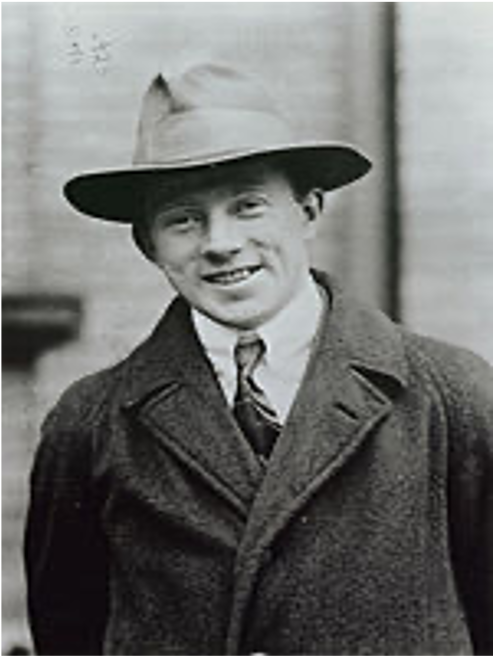
\includegraphics[width=0.25\textwidth]{figs/hesb.png}   
    \end{wrapfigure}
    维尔纳·海森堡(Werner Heisenberg,1901年12月5日-1976年2月1日),德国物理学家,1932年诺贝尔物理学奖。主要贡献:(1) 创立矩阵力学(量子力学的矩阵形式);(2)提出“测不准原理”;(3)散射(S)矩阵。 (学术伦理)
\end{frame}

\begin{frame} [allowframebreaks=]
    \begin{tcolorbox2}{不确定性关系式表明:}
    \begin{itemize}
        \Item 若两力学量算符不对易(对易子不等于零),对易子平均值的平方一般会大于零,则它们的不确定度的积必大于零,说明它们一般不能同时具有确定值
        \Item 若两个力学量算符对易,则总可以找出这样的态(比如共同的本征态),使它们同时有确定值。 
        \Item 
    \end{itemize}   
    \end{tcolorbox2}
\end{frame} 

\begin{frame} [allowframebreaks=]
    TIPS:下列说法,正确的有:
    \begin{enumerate}
        \Item 两力学量算符对易,则同时有确定值。 
        \Item 两力学量算符不对易,则不可能同时有确定值 
        \Item 若两力学量算符有共同的本征态,则彼此对易
        \Item 若两力学量算符不对易,则没有共同本征态
        \Item 若两力学量算符A,B对易,则A的本征函数必是B的本征函数.
        \Item 若[A,B]=常数,则A和B能有共同本征态
    \end{enumerate} 
\end{frame} 

\begin{frame} {}
    \begin{tcolorbox2}{课堂作业2}
     A wavefunction is given by \[ \psi(x,0)=A\left(a^2-x^2\right); \qquad -a<x<a \]
    and zero elsewhere.\\
    find A \\
    find $<x>$\\
    find $<x^2>$\\
    find $<p_x>$\\
    find $<p_x^ 2>$\\
    and verify the uncertainty principle. \\
    \end{tcolorbox2}
\end{frame} 

\begin{frame} 
    \frametitle{}
    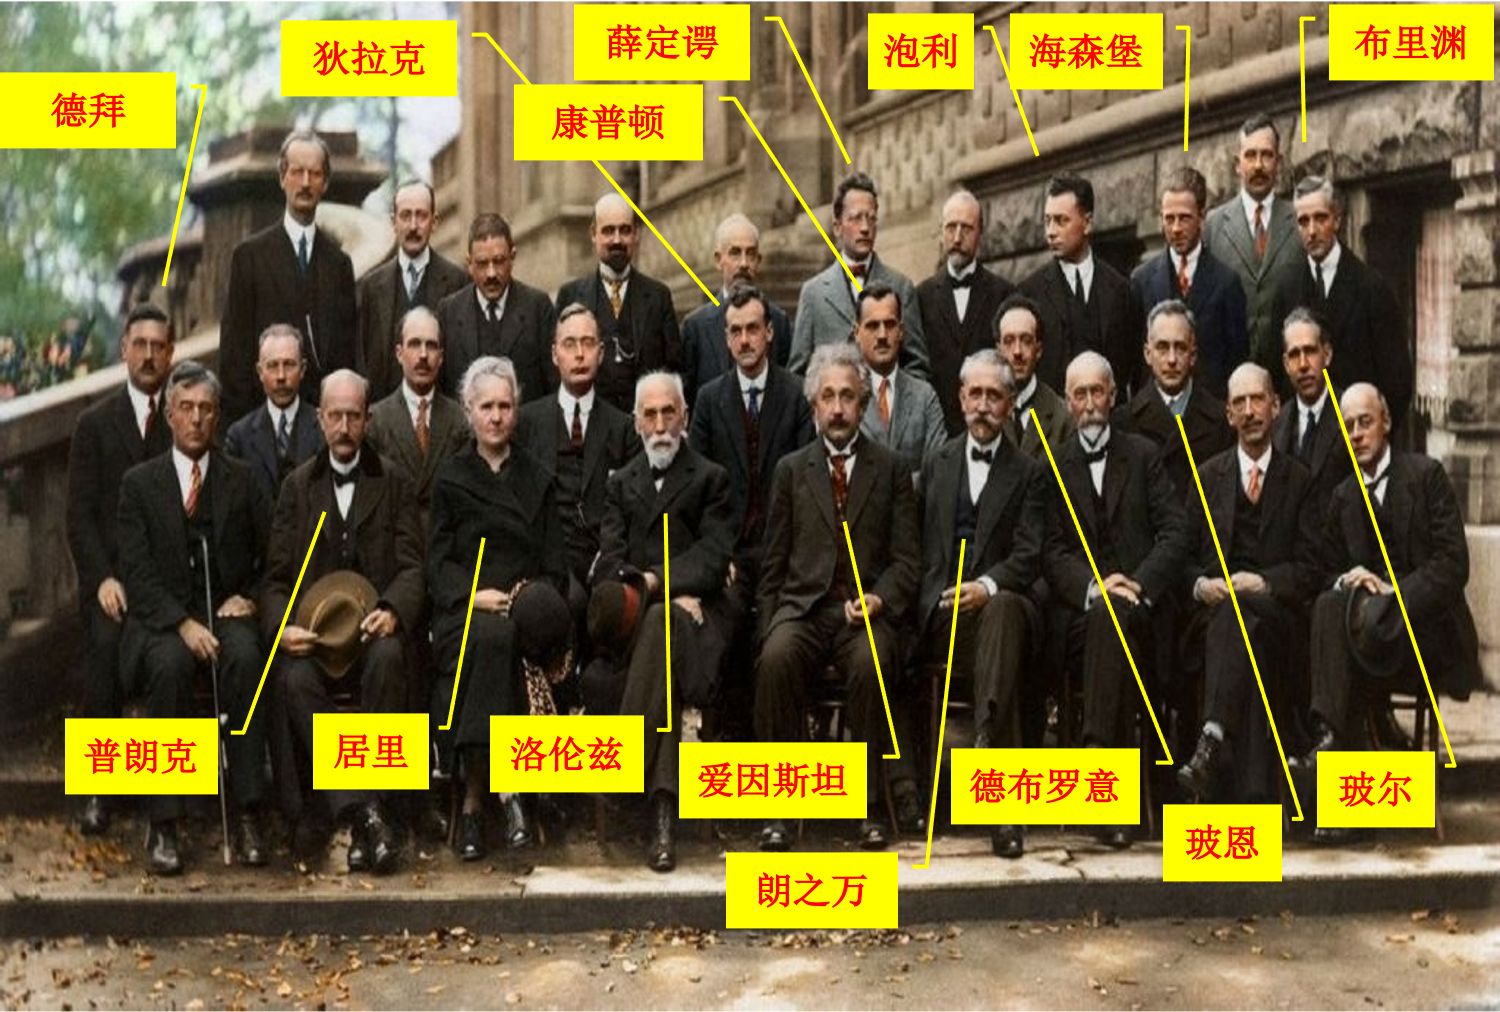
\includegraphics[width=0.9\textwidth]{figs/meet.png}
\end{frame} 

%%%%%%%%%%%%%%%%%%%%%%%%%%%%%%%%%%%%%%%%%%%%%%%%%%%%%%%%%%%%%%%%%%%
\begin{frame}
    \frametitle{课外作业}
    \begin{enumerate}
        \item 已知$[L_x, L_y]=i\hbar L_z$, 试计算体系处于$L_z$的基态 $$Y_{00}=\frac{1}{\sqrt{4\pi}}$$时,$L_x, L_y$的不确定度,并验证不确定性原理.
        \item 试用不确定性原理,估算氢原子基态能量和一维谐振子的最小能量
        \item 设电子在一个原子大小的无限深球型势阱中运动时,求其最小能量.
    \end{enumerate}
\end{frame}
%%%%%%%%%%%%%%%%%%%%%%%%%%%%%%%%%%%%%%%%%%%%%%%%%%%%%%%%%%%%%%%%%%%

\begin{frame}
    \frametitle{}
       4. 已知体系的力学量A有两个本征态$\rs{a_1}, \rs{a_1}$, B也有两个本征态$\rs{b_1}, \rs{b_1}$.它们之间的关系如下, 试求: \\
        \[ \begin{cases}
            &\rs{a_1} =\frac{1}{2} \rs{b_1} +  \sqrt{\frac{3}{4}} \rs{b_2} \\
            &\rs{a_2} =\sqrt{\frac{1}{2}} \rs{b_1} +  \sqrt{\frac{1}{2}} \rs{b_2} 
        \end{cases} \]
        (1) 若测量A发现测量值为 $a_1$, 则再测B时的平均值是多少\\
        (2) 若上问中某次测得值是 $b_1$, 则再试测量A的值为$a_1$的概率是多少?
\end{frame}
%%%%%%%%%%%%%%%%%%%%%%%%%%%%%%%%%%%%%%%%%%%%%%%%%%%%%%%%%%%%%%%%%%%


\section{6.算符运动方程}

\begin{frame}
    \frametitle{前情回顾}
    \begin{itemize}
        \Item 希尔伯特空间的态矢量描述体系状态
        \Item 希尔伯特空间的算符给出体系的物理量
        \Item 算符的本征函数系构成正交归一完全基
        \Item 常见算符本征方程求解
        \Item 算符对易关系及其物理含义 
    \end{itemize}   
\end{frame} 

\subsection{守恒量及守恒条件}

\begin{frame}
\includegraphics[width=0.6\textwidth]{figs/2021-12-17-21-25-13.png} \\
1918年 德国数学家 A. E. Noether : 从自然界的每一对称性可
得到一守恒律;反之,每一个守恒律均揭示蕴含其中的一种对称性。
\end{frame} 

\begin{frame} 
    \frametitle{守恒量定义}
    \begin{enumerate}
        \Item  经典物理中的守恒量与对称条件\\
                守恒量:力学量的值不随时间变化\\
                \begin{itemize}
                    \Item 机械能空间平移不变→动量守恒
                    \Item 机械能空间转动不变→角动量守恒
                    \Item 机械能时间平移不变→能量守恒
                \end{itemize}
        \Item  量子力学中的守恒量\\
                守恒量:在任意态下力学量的平均值不随时间变化\\
                $$ \bar{F}(t)=(\Psi(t), F\Psi(t)) =c.  $$
                守恒量及守恒条件... 
    \end{enumerate}
\end{frame} 

\begin{frame}
    由平均值公式  
        \begin{equation*}
            \begin{split} 
            \bar{F}(t)&=(\Psi(t), F(t)\Psi(t)) \\
            \frac{d\bar{F}}{dt}&=(\frac{\partial\Psi }{\partial t}, F\Psi) +(\Psi, \frac{\partial F }{\partial t}\Psi) +(\Psi, F\frac{\partial\Psi }{\partial t}) \\
            &= - \frac{1}{i\hbar} (H\Psi, F\Psi)+(\Psi, \frac{\partial F }{\partial t}\Psi) + \frac{1}{i\hbar} (\Psi, FH\Psi) \\
            &= - \frac{1}{i\hbar} (\Psi, HF\Psi)+(\Psi, \frac{\partial F }{\partial t}\Psi) + \frac{1}{i\hbar} (\Psi, FH\Psi) \\
            &= (\Psi, \frac{\partial F }{\partial t}\Psi)  +\frac{1}{i\hbar} (\Psi, [F,H]\Psi) \\
            &=\overline{(\frac{\partial F }{\partial t})}  +\frac{1}{i\hbar} \overline{[F,H]} \\
            \end{split}  
        \end{equation*}
    \end{frame} 

\begin{frame}
    \frametitle{算符运动方程}  
        \[\boxed{\frac{d\bar{F}}{dt} = \overline{(\frac{\partial F }{\partial t})}  +\frac{1}{i\hbar} \overline{[F,H]}}\]
\end{frame} 

\begin{frame} 
        \frametitle{守恒条件} 
        由守恒量定义:   
        $$ \bar{F}(t)=(\Psi(t), F\Psi(t)) =c.  $$
        $$\frac{d\bar{F}}{dt}=\overline{(\frac{\partial F }{\partial t})}  +\frac{1}{i\hbar} \overline{[F,H]}=0$$
        得守恒量条件:
        $$\left\{\begin{aligned}
            &\frac{\partial F }{\partial t}=0\\
            &[F,H]=0 \\
        \end{aligned} \right. $$
\end{frame}

\subsection{守恒量性质}

\begin{frame} 
    \frametitle{守恒量性质1} 
    \例[1.试证明守恒量测量值的概率分布不随时间改变]{}
    \证~ F是守恒量,则 $[F,H]=0$, 设F,H的共同本征函数系$\{\varphi_n\}$, 有:\\ 
    任意态$\Psi(t)$在$\{\varphi_n\}$展开,其展开系数为:
    $$C_n(t)=(\varphi_n, \Psi(t))$$
    展开系数的模方即为测量值为本征值$f_n$的概率,因此要证明:
    $$\frac{d}{dt} |C_n(t)|^2=0$$
\end{frame}

\begin{frame} [allowframebreaks=]
    $$\begin{aligned}
      \frac{d}{dt} |C_n(t)|^2 &= \frac{d}{dt} C_n^* C_n \\
      &=C_n \frac{d}{dt} C_n^*  +  C_n^*\frac{d}{dt}C_n \\
      &=[C_n^*[\frac{d}{dt} C_n]^*  +  [C_n^*\frac{d}{dt}C_n] \\
    \end{aligned}$$
    $$\begin{aligned}
      C_n^*\frac{d}{dt}C_n&= (\varphi_n, \Psi)^* \frac{d}{dt}(\varphi_n, \Psi) \\
      &= (\varphi_n, \Psi)^* (\varphi_n, \frac{d}{dt}\Psi) \\
      &= \frac{1}{i\hbar}(\varphi_n, \Psi)^* (\varphi_n, H\Psi) \\
      &= \frac{1}{i\hbar}(\varphi_n, \Psi)^* (H\varphi_n, \Psi) = \frac{E_n}{i\hbar}C_n ^* C_n 
    \end{aligned}$$
    $$\begin{aligned}
        \frac{d}{dt} |C_n(t)|^2 &= [C_n^*[\frac{d}{dt} C_n]^*  +  [C_n^*\frac{d}{dt}C_n] \\
        &= [\frac{E_n}{i\hbar}C_n ^* C_n ]^* + \frac{E_n}{i\hbar}C_n ^* C_n \\
        &= -\frac{E_n}{i\hbar}C_n ^* C_n ] + \frac{E_n}{i\hbar}C_n ^* C_n \\
        &=0
    \end{aligned}$$
      证毕! \\
    \Tips ~无论体系处于本征态还是叠加态(任意态),守恒量的平均值及各测量值的概率分布都不随时间变化。         
\end{frame}

\begin{frame}
    \frametitle{性质2}
    \例[2.试证明若体系有两个不对易守恒量,则一般存在简并能级]{}
    \证~ 设F、G都是体系的守恒量,则有 $[F,H]=0$, $[G,H]=0$, 设F,H的共同本征函数系$\{\varphi_n\}$, 有:\\ 
    $$F\varphi_n =f_n \varphi_n, \qquad H\varphi_n =E_n \varphi_n $$
    $$H(G\varphi_n) =HG\varphi_n=GH\varphi_n= E_n (G\varphi_n)$$
    说明 $G\varphi_n$ 和 $\varphi_n$ 都是H的属于$E_n$的本征态。
    假设能级非简并,则$G\varphi_n$ 和 $\varphi_n$描述同一个态,两者最多只差一个常数因子,设为 $g_n$,有:
    $$G\varphi_n=g_n \varphi_n$$
    也就是说,$\varphi_n$也是G的本征态,即 F和G具有相同的本征函数系,即它们对易,与题设相矛盾。评毕!\\
\end{frame}

\begin{frame}
    \begin{tcolorbox2}{推论:}
        若体系有两个不对易守恒量,则一般存在简并能级, 非简并能级都是守恒量的本征态,简并能级中存在守恒量的一个本征态。\\
        根据能级简并,可找出体系的守恒量;根据能级不简并,可找到守恒量的本征态。
    \end{tcolorbox2}
\end{frame}

\subsection{常见守恒定律}

\begin{frame} 
    \frametitle{动量守恒} 
    \例[3.试证明自由粒子的动量是守恒量]{}                                   
    \证~ (1)自由粒子动量算符为:
    $$ \hat{\vec{p}} = -i\hbar\nabla  $$
    不显含时间,有 $$\frac{d}{dt}\hat{\vec{p}}=0$$ 
    (2), 自由粒子哈密顿算符为: $$ \hat{H} = \frac{1}{2\mu} \hat{\vec{p}}^2 $$
    $$\begin{aligned}
        [\hat{\vec{p}},\hat{H}]&= \frac{1}{2\mu}[\hat{\vec{p}}, \hat{\vec{p}}^2 ] =0 \\
    \end{aligned}$$
    证毕!
\end{frame}

\begin{frame} 
    \frametitle{} 
    \例[4.试证明空间平移不变性导致动量守恒]{}                                
    \证~ (1)设体系沿x轴方向无穷小平移a:
    $$ T(a)\psi(x)=\psi(x-a) $$
    做Taylor展开,可求得
    \[\begin{aligned}
        \psi(x-a)=&\psi(x) -a \frac{d}{d x} \psi(x)+\frac{a^{2}}{2 !} \frac{d^{2}}{d x^{2}} \psi(x)-\ldots \\
        &=e^{-a \frac{d}{d x}} \psi(x) \\
    T(a)=&e^{-a \frac{d}{d x}}= e^{-\frac{i}{\hbar}a \hat{p}_x}\\
        &=1-\frac{i}{\hbar}a \hat{p}_x 
    \end{aligned}\]   
 $$T(\delta x)= e^{-\frac{i}{\hbar}\delta x p_x } $$ 
\end{frame}

\begin{frame}    
    推广到三维,有:
    $$ T(\delta \hat{\vec{r}})= e^{-\frac{i}{\hbar}\delta \hat{\vec{r}}\cdot \hat{\vec{p}} }  $$ 
    对于无穷小平移,有:
    $$T=1-\frac{i}{\hbar}\delta x p_x$$
    很明显,平移算符不显含时间,满足条件(1)\\
    (2)若具空间平移不变性,则
    $$\begin{aligned}
        [T,H]&= 0 \\
        [1-\frac{i}{\hbar}\delta x p_x, H] &=0 \\
        [1, H]-[\frac{i}{\hbar}\delta x p_x, H]&=0 \\
        [\frac{i}{\hbar}\delta x p_x, H]&=0 \\
        [p_x, H] &=0 \\
    \end{aligned}$$
    证毕!
\end{frame}

\begin{frame}
    \frametitle{角动量守恒} 
    \例[5.试证明在中心力场中运动粒子的角动量是守恒量]{}                                
    \证~ (1)中心力场中的角动量
    $$
    \left\{\begin{array}{l}
        \hat{L}_{x}=i \hbar\left[\sin \varphi \frac{\partial}{\partial \theta}+\cot \theta \cos \varphi \frac{\partial}{\partial \varphi}\right] \\
        \hat{L}_{y}=-i \hbar\left[\cos \varphi \frac{\partial}{\partial \theta}+\cot \theta \sin \varphi \frac{\partial}{\partial \varphi}\right] \\
        \hat{L}_{z}=-i \hbar \frac{\partial}{\partial \varphi}
        \end{array}\right.
    $$
    $$ \hat{L}^{2}=-\hbar^{2}\left[\frac{1}{\sin \theta} \frac{\partial}{\partial \theta}\left(\sin \theta \frac{\partial}{\partial \theta}\right)+\frac{1}{\sin ^{2} \theta} \frac{\partial^{2}}{\partial \varphi^{2}}\right] $$
    
    很明显,角动量不显含时间,满足条件(1)\\
\end{frame}

\begin{frame} 
    (2) 中心力场哈密顿算符为: 
    $$
    \hat{H}=-\frac{\hbar^{2}}{2 \mu r^{2}}\left[\frac{\partial}{\partial r}\left(r^{2} \frac{\partial}{\partial r}\right)+\frac{1}{\sin \theta} \frac{\partial}{\partial \theta}\left(\sin \theta \frac{\partial}{\partial \theta}\right)+\frac{1}{\sin ^{2} \theta} \frac{\partial^{2}}{\partial \varphi^{2}}\right]+U(r)
    $$
    $$
    \hat{H}=-\frac{\hbar^{2}}{2 \mu r^{2}} \frac{\partial}{\partial r}\left(r^{2} \frac{\partial}{\partial r}\right)+\frac{\hat{L}^{2}}{2 \mu r^{2}}+U(r)
    $$
    哈密顿算符与角动量各分量算符及角动量方均对易 因为(a)角动量都是$\theta, \varphi$ 的函数,与$r$无关,与哈密顿算符只含$r$的项对易。
    (b)角动量都与$L^2$对易。\\
    证毕!
\end{frame}

\begin{frame} 
    \frametitle{能量守恒} 
    \例[6.试证明哈密顿算符不显含时间的体系能量守恒]{}                               
    \证~ (1)密顿算符不显含时间:
    有 $$\frac{d}{dt}\hat{H}=0$$ 
    (2), 密顿算符与自己对易: 
        $$ [\hat{H},\hat{H}]=0 $$
    证毕!
\end{frame}

\begin{frame} 
    \frametitle{} 
    \begin{tcolorbox2}{角动量守恒:}
        试证明:具有空间旋转不变性的体系角动量守恒                               
    \end{tcolorbox2}
    对于无穷小平移,有:
    $$T=1-\frac{i}{\hbar}\delta x p_x$$
    同理, 对于无穷小旋转,有:
    $$R(\delta \vec{\theta}) \psi(\vec{r})=e^{-\frac{i}{\hbar} \delta \vec{\theta} \cdot \widehat{\vec{L}}} \psi(\vec{r})
$$
...
\end{frame}

\begin{frame} 
    \begin{tcolorbox2}{能量守恒:}
        试证明:具有时间平移对称性的体系能量守恒                               
    \end{tcolorbox2}
    \begin{tcolorbox2}{宇称守恒:}
        试证明:具有空间反射对称性的体系宇称守恒                             
    \end{tcolorbox2}
\end{frame}

\begin{frame}
    \frametitle{宇称守恒} 
    \例[7.试证明若哈密顿算符空间反射不变,则宇称守恒]{}                               
    \证~ (1)宇称算符:
    空间反射:$$\vec{r} \to -\vec{r} $$
    $$\Psi(\vec{r}) \to \Psi(-\vec{r}) $$
    定义宇称算符: $$ \hat{P}\Psi(\vec{r},t) = \Psi(-\vec{r},t) $$
    
    (2) 解宇称算符本征方程: 
    对于本征函数 $\psi_p (\vec{r})$, 有:
    $$\begin{aligned}
        \hat{P}\psi_p (\vec{r}) &= p\psi_p (\vec{r}) \\
        \hat{P}^2\psi_p (\vec{r}) &= \hat{P} p\psi_p (\vec{r}) = p^2\psi_p (\vec{r})\\
        &= 0
    \end{aligned}$$
\end{frame}

\begin{frame} 
    基于定义,有:
    $$\begin{aligned}
        \hat{P}^2\psi_p (\vec{r}) &= \hat{P} [\hat{P} \psi_p (\vec{r})]\\
        &= \hat{P} \psi_p (-\vec{r})\\
        &= \psi_p (\vec{r})\\
    \end{aligned}$$
    得本征值 $p=\pm 1$,分别称为偶宇称和奇宇称。\\ \vspace{0.6em}
    (3) 证明宇称守恒 \\
    (a) 显然,宇称算符不显含时间t,满足条件(1)\\

\end{frame}

\begin{frame} 
    (b) 当哈密顿算符具有空间反射不变性,即:
    $$ H(\vec{r},t)= H(-\vec{r},t)$$
    对于任意态,有:
    $$\begin{aligned}
        \hat{P} (\hat{H}(\vec{r},t) \Psi (\vec{r},t)) &= \hat{H}(-\vec{r},t) \Psi (-\vec{r},t)\\
        &= \hat{H}(\vec{r},t) \Psi (-\vec{r},t)\\
        &= \hat{H}(\vec{r},t) \hat{P} \Psi (\vec{r},t)\\
    \end{aligned}$$
    得: $$ \hat{P} \hat{H} = \hat{H} \hat{P} $$
    即:$$[\hat{P}, \hat{H}]=0$$
    满足条件(2),证毕!
\end{frame}

\begin{frame}
    \centering
    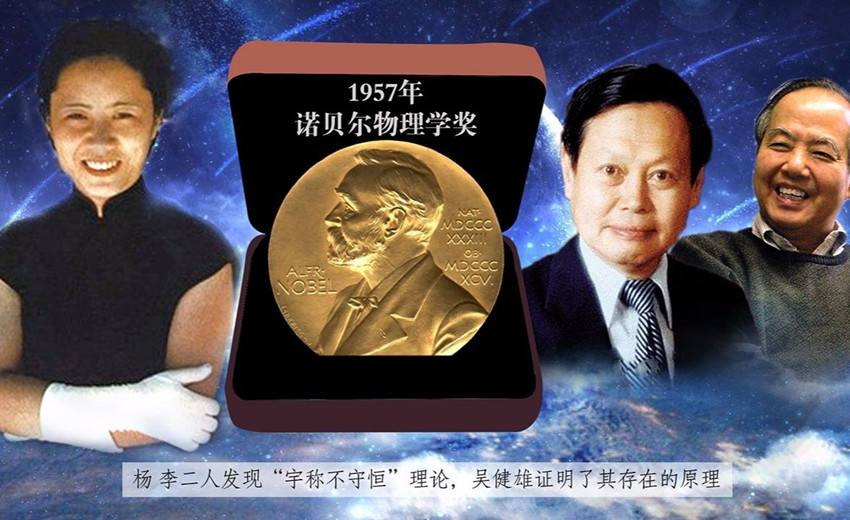
\includegraphics[width=0.8\textwidth]{figs/2021-12-18-00-23-17.png} \\
\end{frame} 

%%%%%%%%%%%%%%%%%%%%%%%%%%%%%%%%%%%%%%%%%%%%%%%%%%%%%%%%%%%%%%%%%%%
\begin{frame}
    \frametitle{课外作业}
    \begin{enumerate}
        \item 试证明具有空间旋转不变性的体系角动量守恒  
        \item 试证明球谐函数$Y_{lm}$的宇称由量子数$l$决定  
        \item 对于一维自由粒子,试证明 \\
                (1)动量,宇称都是守恒量 \\
                (2)动量算子与宇称算子不对易,因此存在能级简并
    \end{enumerate}
\end{frame}
%%%%%%%%%%%%%%%%%%%%%%%%%%%%%%%%%%%%%%%%%%%%%%%%%%%%%%%%%%%%%%%%%%%

